\section{Model}

\noindent The problem presented involves a complicated system that needs to accommodate the mechanics of how a human jumps on an elastic surface in three dimensions. This is a lot of information that needs to be concatenated to create a realistic model so the best approach is to work up from a simple model that reduces the number of parameters and constraints by using assumptions.
\\
\\
\noindent In order to model this system, a two dimensional cross-section of a trampoline was taken, as seen in Figure \ref{fig:flattramp}. This consists of a light, inextensible string between two springs, with spring constant $k$, which stay a constant distance, $L$ apart. 

\begin{figure}[H]
	\centering
	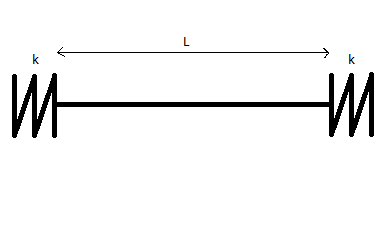
\includegraphics[width=0.6\linewidth, height=2in]{ill1.png}
	\caption{Two-Dimensional model of a trampoline at resting point with no masses added to it.}\label{fig:flattramp}
\end{figure}

\noindent With the purpose of simplifying the model, it was decided to model a person as a point mass. This removes any complications in modelling the jumping motion of a human body. When a mass is added to the system, the string changes shape, causing both springs to stretch. This introduces a potential energy into the system which can be used along with the kinetic and gravitational potential energy of the mass to form an ordinary differential equation, with the use of Lagrangian mechanics, which describes the system \cite{lagrange}. The following Lagrangian equations were used to find the differential equations: 

\begin{equation}
\mathcal{L} = T - V
\end{equation}\label{lagrangeeq1}

\begin{equation}
\frac{d}{dt}\frac{\partial \mathcal{L} }{\partial \dot q_i} - \frac{\partial \mathcal{L} }{\partial q_i} = 0
\end{equation}\label{lagrangeeq2}

\noindent Where $T$ is the kinetic energy in the system, $V$ is the potential energy in the system and $q_i$ are the variables of the system. \\

\noindent For this study, two types of model were created, a one mass and two mass model, discussed in Sections \ref{1mm} and \ref{2mm} respectively. The two mass model can only be used when both masses are in contact with the trampoline and the one mass model can only be used when one mass is in contact with the trampoline. This will occur when the other mass has left the trampoline. It is possible to find when a mass is about to leave the trampoline by calculating when the trampoline has an acceleration that is lower than the acceleration due to gravity, which would cause the mass to detach. %The variable is the displacement of the mass on the trampoline. 
By combining the two models, it is possible to track the maximum heights reached by both masses. 
\\
\\
\noindent The aim of the model is to find the maximum height reached by each of the masses under different initial conditions. This is discussed in Section \ref{results}. It can then be assumed that the severity of the injury increases with height.
%edit

\subsection{One Mass Model}\label{1mm}
\noindent This first step in creating the one mass model is to find a differential equation which represents the system. This is created by looking at Figure \ref{fig:system1}.

\begin{figure}[H]
	\centering
	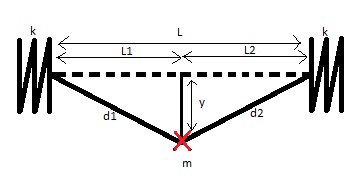
\includegraphics[width=0.6\linewidth, height=1.6in]{system1.png}
	\caption{Initial trampoline model with human modelled as point mass positioned centrally on trampoline.}\label{fig:system1}
\end{figure}

\noindent Where:
\begin{itemize}
\item $m$ [kg] is the mass.
\item $L_1$ [m] is the horizontal length from the left spring to the mass.
\item $L_2$ [m] is the horizontal length from the right spring to the mass.
\item $y$ [m] is the displacement of the mass.
\item $d_1$  [m] is the length of the string from the left spring to the mass.
\item $d_2$  [m] is the length of the string from the right spring to the mass.
\end{itemize}




\noindent As can be seen, there are a number of different parameter values which affect the system. For the purpose of this model, parameters $L_1$ and $L_2$ are kept constant. By using these constants, it is possible to find the other parameters in terms of the variable, y. \\

\noindent Since $L_1$, $y$ and $d_1$, and $L_1$, $y$ and $d_2$ both are right angled triangles, Pythagoras' theorem \cite{pythagoras} can be used to find $d_1$ and $d_2$: 

\begin{equation}
d_1 = \sqrt{L_{1}^{2} + y^{2}},\,\,\,\,\,\,\, d_2 = \sqrt{L_{2}^{2} + y^{2}}
\end{equation}

\noindent It is then possible to sum $d_1$ and $d_2$ to find the new length of the trampoline surface when the mass is connected. This means that the stretch in the two springs must be the new length of the trampoline surface minus the distance between the springs ($L$). So the distance each spring is stretched by, $\Delta x$, can found using the following equation:

\begin{equation}
\Delta x = \frac{1}{2}\left[\middle(d_{1}+d_{2}\middle)-L\right] 
\end{equation}

\noindent It is now possible to find all of the kinetic and potential energies in the system and therefore use the Lagrange equations (Equation (1) and Equation (2)) to find a differential equation which describes the system. \\

\noindent The mass provides both a kinetic energy ($\frac{1}{2}m\dot{y}^2$) \cite{kinetic} and a gravitational potential energy ($mgy$) \cite{potentiale} to the system and the trampoline provides a elastic potential energy to the system ($\frac{1}{2}k\Delta x^2$) \cite{potentiale} from each spring. This means that:
%http://www.physicsclassroom.com/class/energy/Lesson-1/Kinetic-Energy
%http://www.physicsclassroom.com/class/energy/Lesson-1/Potential-Energy

\begin{equation}
T = \frac{1}{2}m\dot{y}^{2}
\end{equation}

\noindent and

\begin{equation}
V = k\Delta x^{2}-mgy
\end{equation}

\noindent So, using Equation (1)

\begin{equation}
\mathcal{L} = \frac{1}{2}m\dot{y}^{2}-k\Delta x^{2}+mgy
\end{equation}
%calculated from equation (ref lagrange1)

\noindent Now, Equation (2) can be used to find a differential equation which describes the system:

\begin{equation}
\frac{d}{dt}\frac{\partial\mathcal{L}}{\partial\dot{y}} = m\ddot{y}
\end{equation}

\noindent and

\begin{equation}\\
\frac{\partial\mathcal{L}}{\partial y} = -2k\Delta x  \frac{d\Delta{x}}{dy} + mg 
\end{equation}

\noindent where

\begin{equation}
\frac{\partial\Delta x}{\partial y} = \frac{1}{2}\left(\frac{y}{d_1}+ \frac{y}{d_2}\right)
\end{equation}

\noindent Combining (8), (9) and (10) gives the terms seen in the Lagrange Equation (2):

\begin{equation}
m\ddot{y} + 2k \Delta x \frac{\partial \Delta x}{\partial y}- mg = 0
\end{equation}
%this is the differential equation produced, ref lagrange 2.

\noindent With this differential equation, it is possible to set an initial position of the mass on the trampoline and an initial velocity at that point, then the position and velocity of the mass are tracked over time until the mass leaves the surface of the trampoline. An example of the change in position and velocity can be seen in Figure \ref{fig:1MM_Disp_Vel}.

\begin{figure}[H]
	\centering
    \begin{subfigure}{0.45\textwidth}
		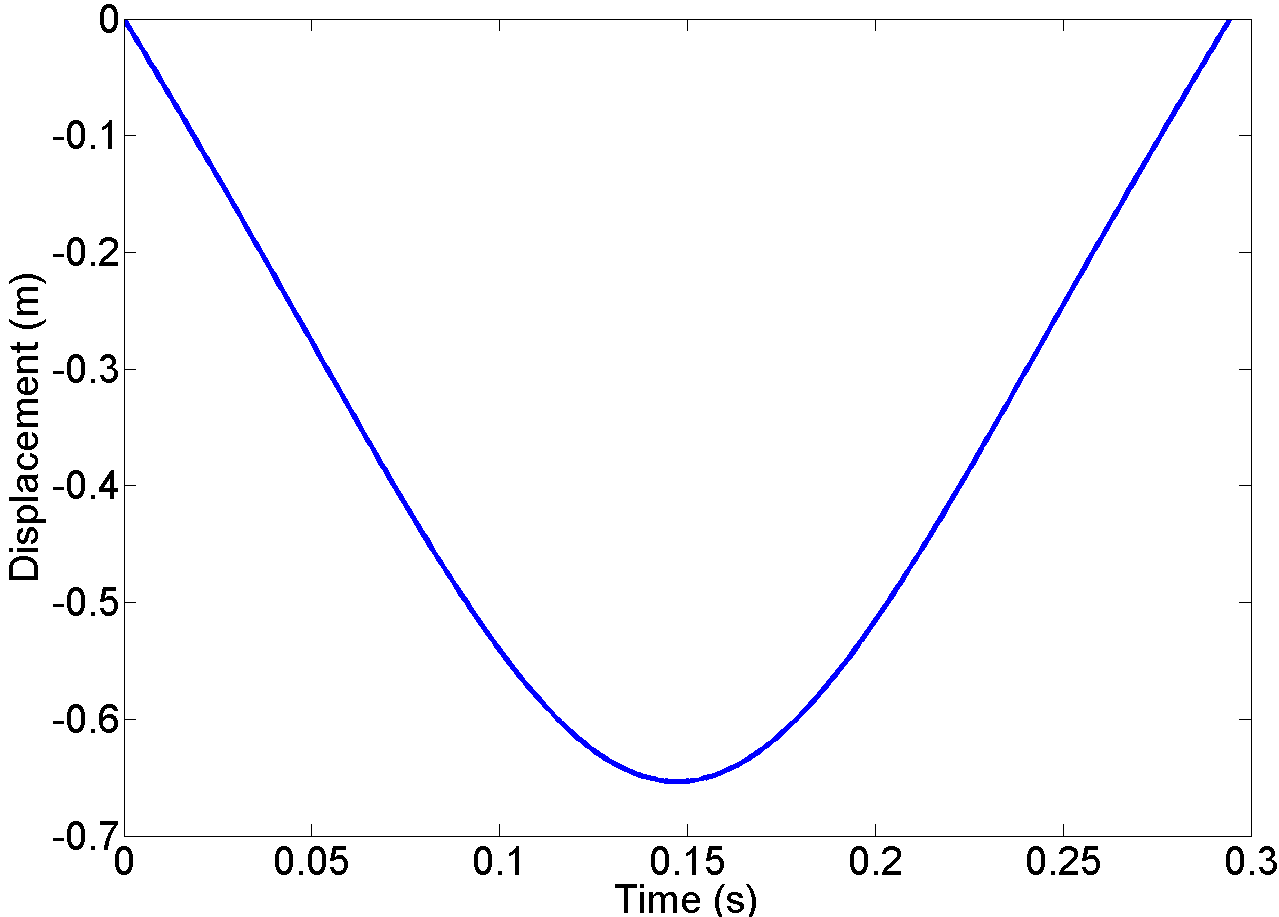
\includegraphics[width=\textwidth]{1MM_Disp.png}
    	\caption{The displacement of the mass while on the trampoline.}\label{fig:1MM_Disp}
    \end{subfigure}\hfill
	\begin{subfigure}{0.45\textwidth}
		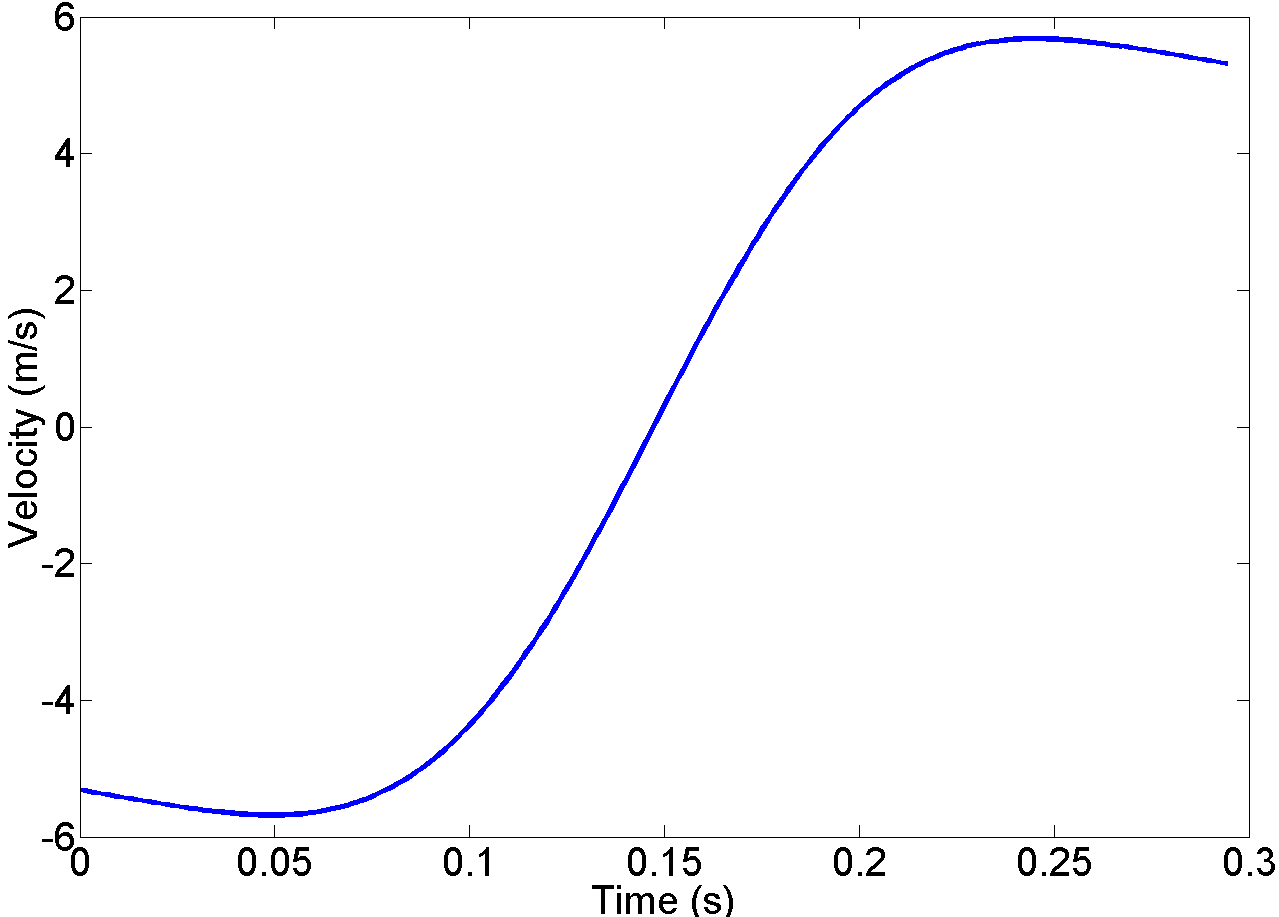
\includegraphics[width=\textwidth]{1MM_Vel.png}
    	\caption{The velocity of the mass while on the trampoline.}\label{fig:1MM_Vel}
    \end{subfigure}\hfill
    \caption{The displacement and velocity of a 50kg mass, in the center of a 3m long trampoline with a spring constant of 77500N/m, dropped from 1.4m. }\label{fig:1MM_Disp_Vel}
\end{figure}

\noindent By taking the position and velocity of the mass when it leaves the trampoline, it is possible to find the maximum height the mass will reach using the following equation:

\begin{equation}
h = y_{final} + s
\end{equation}

\noindent Where $y_{final}$ the displacement of the mass when it leaves the trampoline and $s$ is calculated from one of the equations of motion \cite{suvat}:

\begin{equation}
s = \frac{-u^2}{2g}
\end{equation}

\noindent Where $u$ is the velocity of the mass when it leaves the trampoline. \\

\noindent The maximum height reached can then by used to determine the severity of the injury the person experiences if they were to fall from that height above the trampoline. 

\subsubsection{Parameter Tests}\label{parametertests}
In order to see the effects different parameters have on the system a number of tests were derived which look at the relationships between the different parameters and the minimum point of the mass on the trampoline, the total time spent on the trampoline and the maximum height reached by the mass. The parameters tested were the spring constant ($k$), the total length of the trampoline ($L$), the distance between the mass and the left edge of the trampoline ($L_1$), the starting height of the mass before it comes into contact with the trampoline, and the mass of the mass. For each test, all of the other parameters are kept constant and only the parameter in question is varied.

\paragraph{Spring Constant ($k$)}\mbox{}\\

\begin{figure}[H]
	\centering
    \begin{subfigure}[t]{0.3\textwidth}
		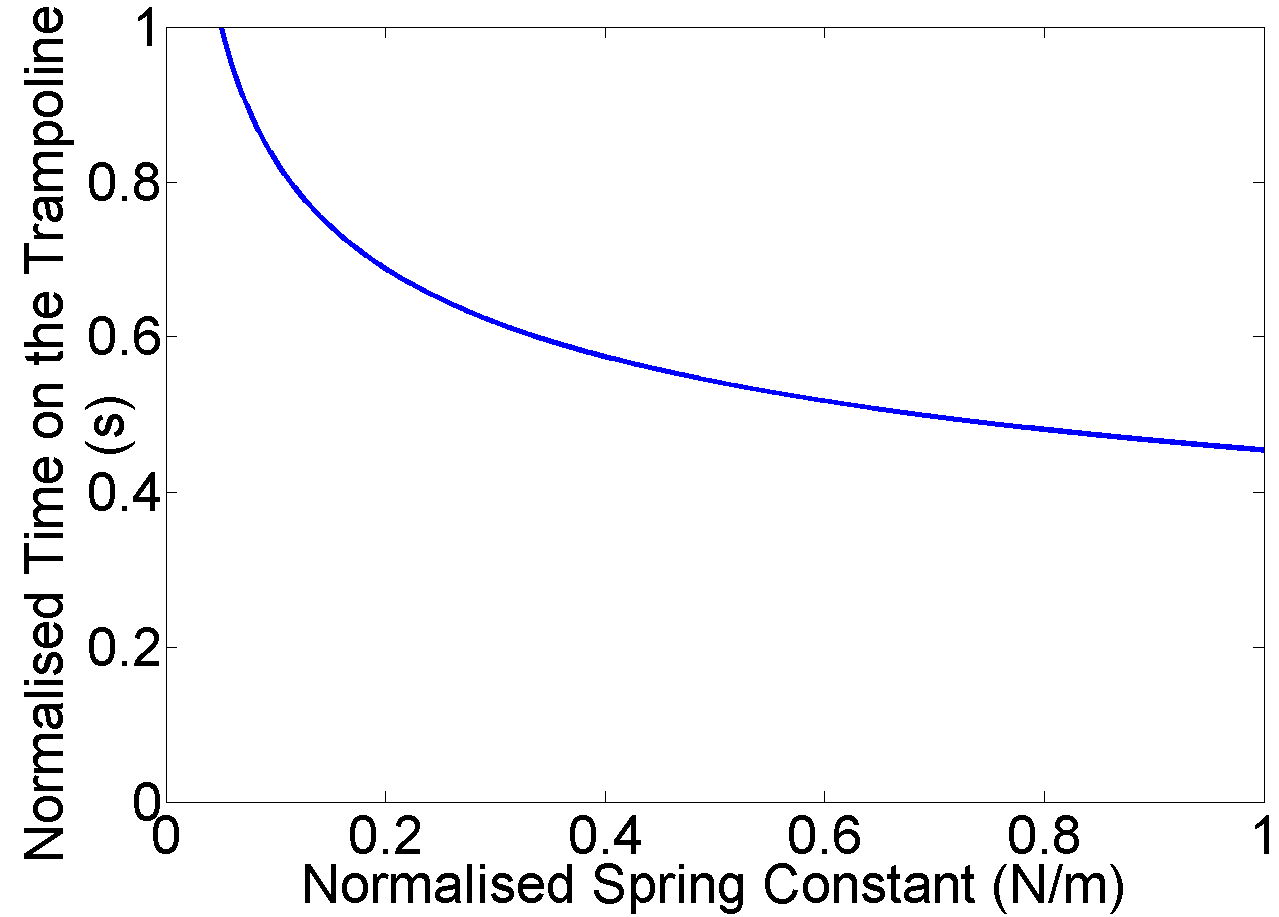
\includegraphics[width=\textwidth]{Norm_Time_Spring.png}
    	\caption{Time spent on trampoline.}\label{fig:Norm_Time_Spring}
    \end{subfigure}\hfill
	\begin{subfigure}[t]{0.3\textwidth}
		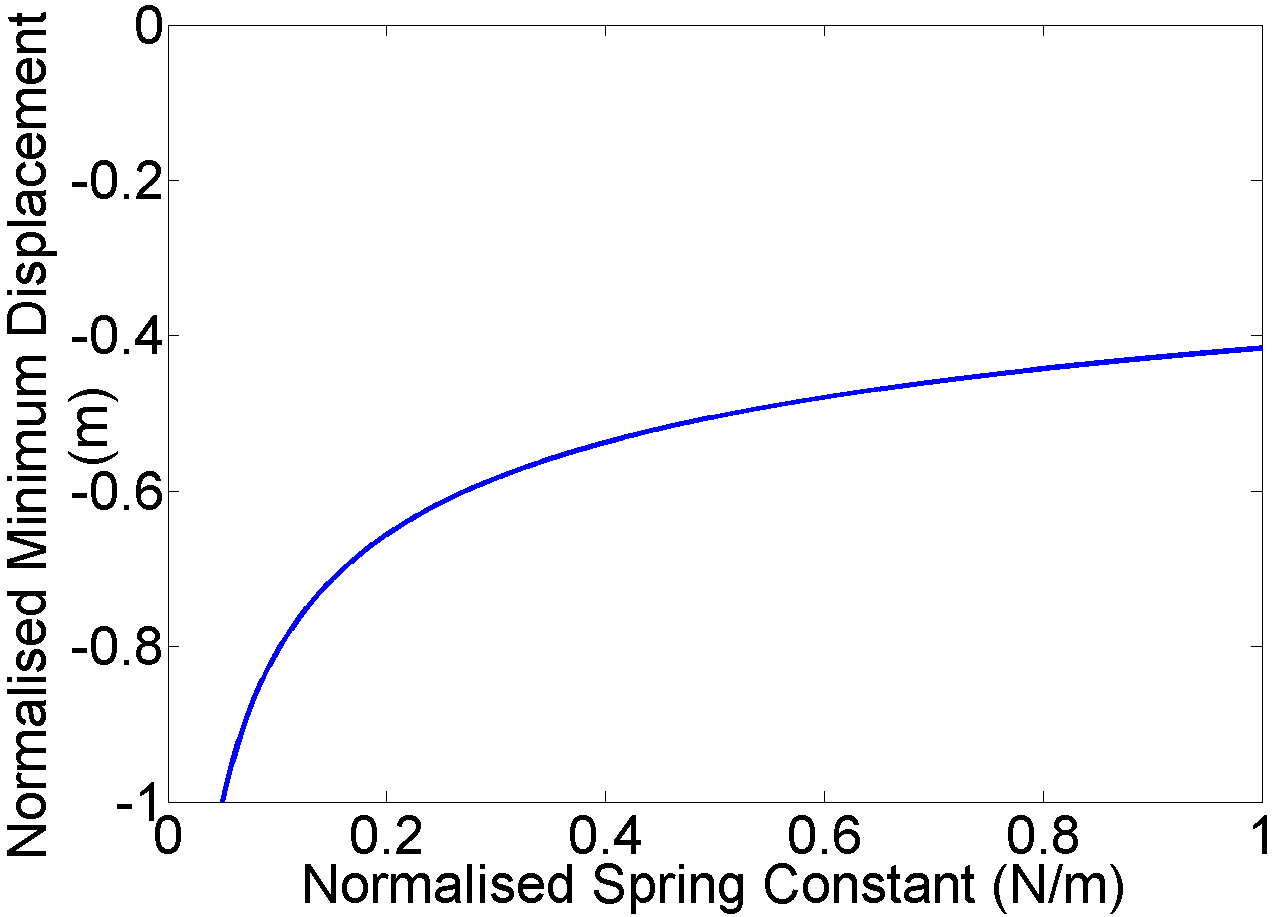
\includegraphics[width=\textwidth]{Norm_MinY_Spring.png}
    	\caption{Most negative displacement reached by the mass on the trampoline.}\label{fig:Norm_MinY_Spring}
    \end{subfigure}\hfill
    \begin{subfigure}[t]{0.3\textwidth}
		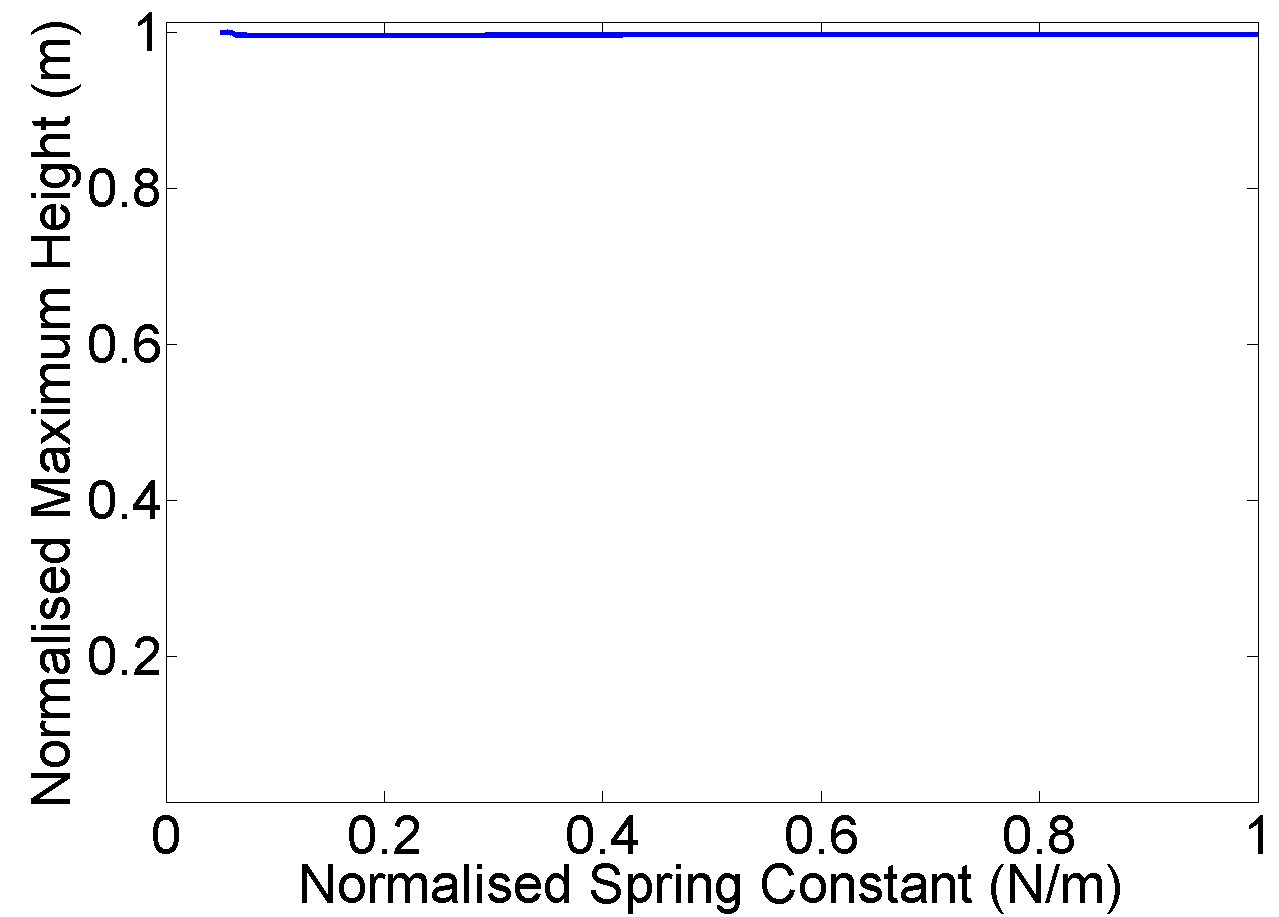
\includegraphics[width=\textwidth]{Norm_Height_Spring.png}
    	\caption{Maximum height reached after leaving the trampoline.}\label{fig:Norm_Height_Spring}
    \end{subfigure}\hfill
    \caption{How the spring constant $k$ affects the other parameters when kept constant.}\label{fig:Norm_Spring}
\end{figure}

\noindent Figure \ref{fig:Norm_Time_Spring} shows that the higher the spring constant, the less time that is spent of the trampoline. This follows an inverse exponential pattern, which means that the amount of time spent on the trampoline converges to an asymptote as the spring constant increases. 
As can be seen from Figure \ref{fig:Norm_MinY_Spring} the displacement and spring constants have a logarithmic relationship with some convergence.
As Figure \ref{fig:Norm_Height_Spring} shows the maximum height that the mass can reach is unchanged as the spring constant increases. This means that the spring constant has no effect on the height. 


\paragraph{Total Length of the Trampoline ($L$)}\mbox{}\\

\begin{figure}[H]
	\centering
    \begin{subfigure}[t]{0.3\textwidth}
		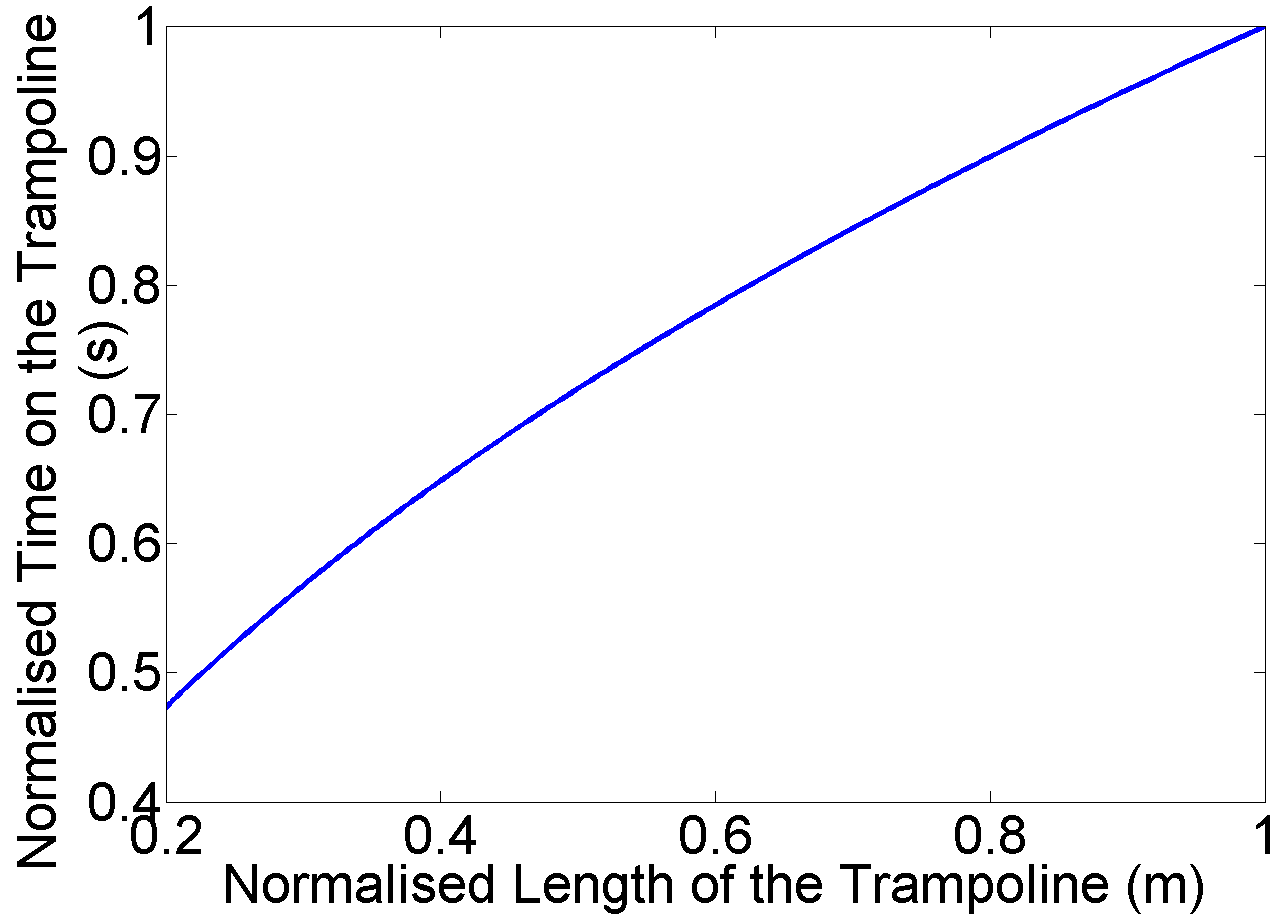
\includegraphics[width=\textwidth]{Norm_Time_LengthTramp.png}
    	\caption{Time spent on trampoline.}\label{fig:Norm_Time_LengthTramp}
    \end{subfigure}\hfill
	\begin{subfigure}[t]{0.3\textwidth}
		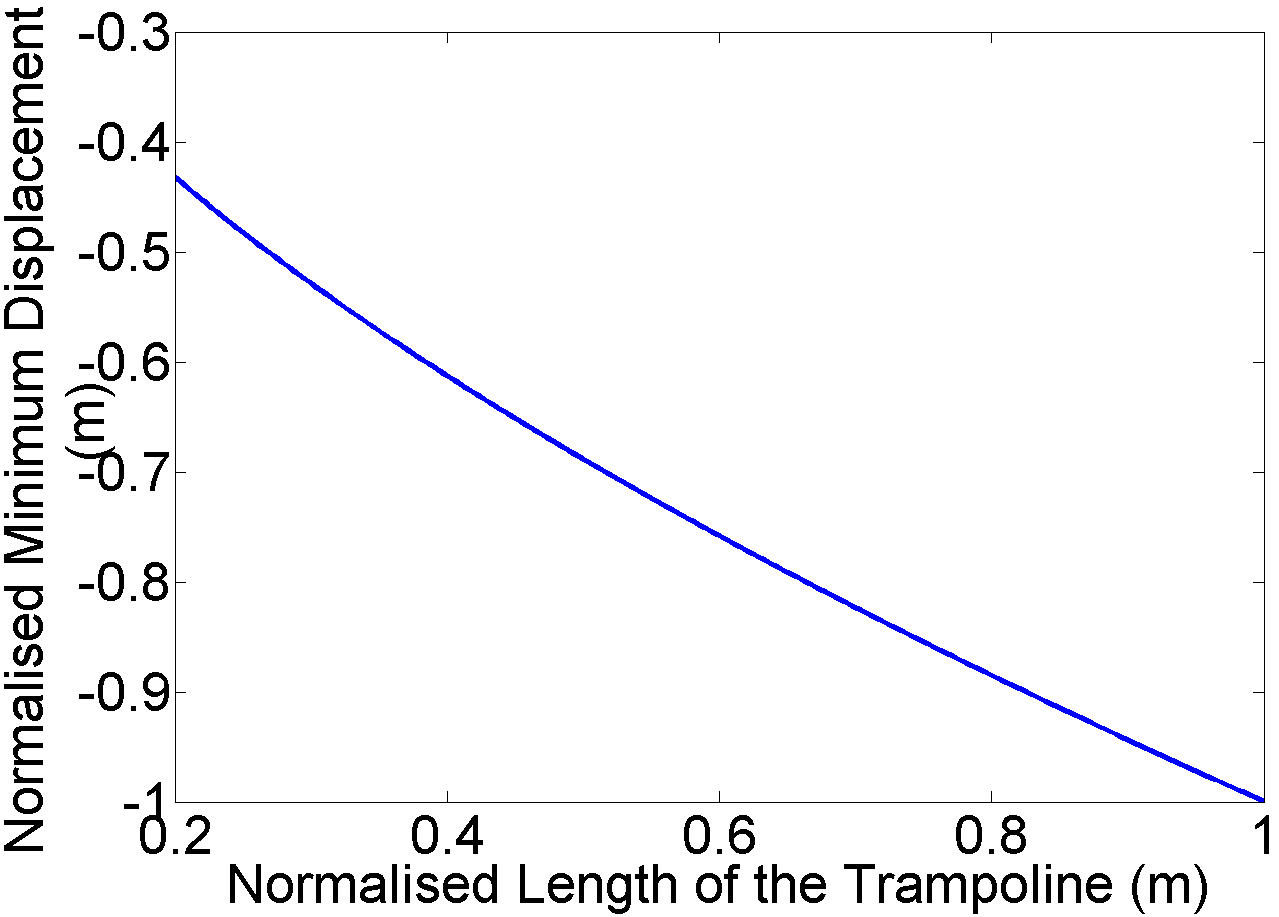
\includegraphics[width=\textwidth]{Norm_MinY_LengthTramp.png}
    	\caption{Most negative displacement reached by the mass on the trampoline.}\label{fig:Norm_MinY_LengthTramp}
    \end{subfigure}\hfill
    \begin{subfigure}[t]{0.3\textwidth}
		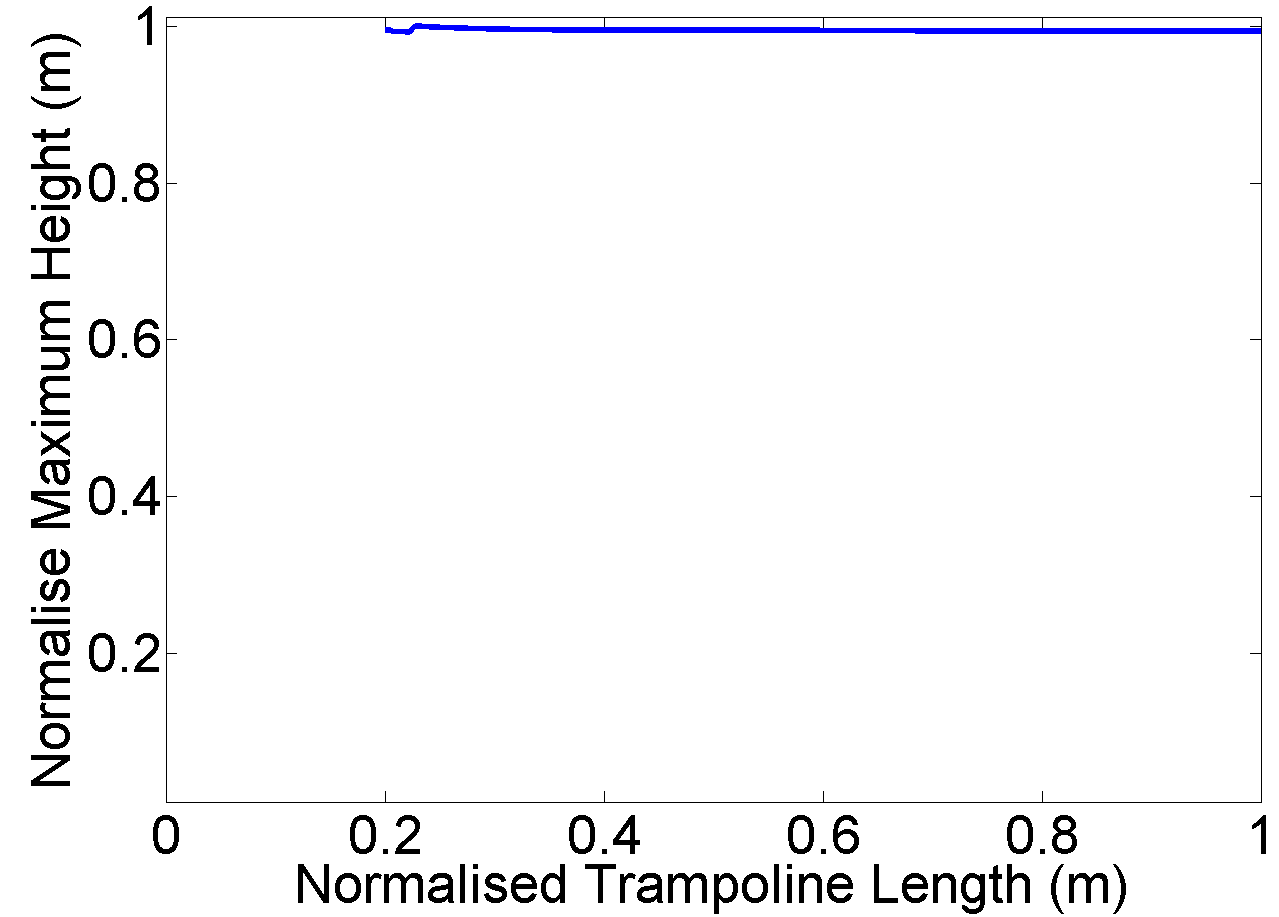
\includegraphics[width=\textwidth]{Norm_Height_LengthTramp.png}
    	\caption{Maximum height reached after leaving the trampoline.}\label{fig:Norm_Height_LengthTramp}
    \end{subfigure}\hfill
    \caption{How the length of the trampoline $L$ affects the other parameters when kept constant.}\label{fig:Norm_LengthTramp}
\end{figure}


\noindent Figure \ref{fig:Norm_Time_LengthTramp} shows a linear relationship between the length of the trampoline and the time spent on it. This means that the larger the trampoline is, the longer that the mass will stay attached before leaving. 
The minimum distance that the trampoline will descend has a negative linear relationship with the length of the trampoline, so the longer the trampoline, the higher the trampoline will stay, as can be seen from Figure \ref{fig:Norm_MinY_LengthTramp}.
Figure \ref{fig:Norm_Height_LengthTramp} shows how the length of the trampoline effects the maximum height that the mass reaches. There is no effect, meaning that regardless of how long the trampoline is, the mass will always reach the same height regardless of changes in this parameter.



\paragraph{Distance of the Mass from the Left Edge of the Trampoline ($L_1$)}\mbox{}\\

\begin{figure}[H]
	\centering
    \begin{subfigure}[t]{0.3\textwidth}
		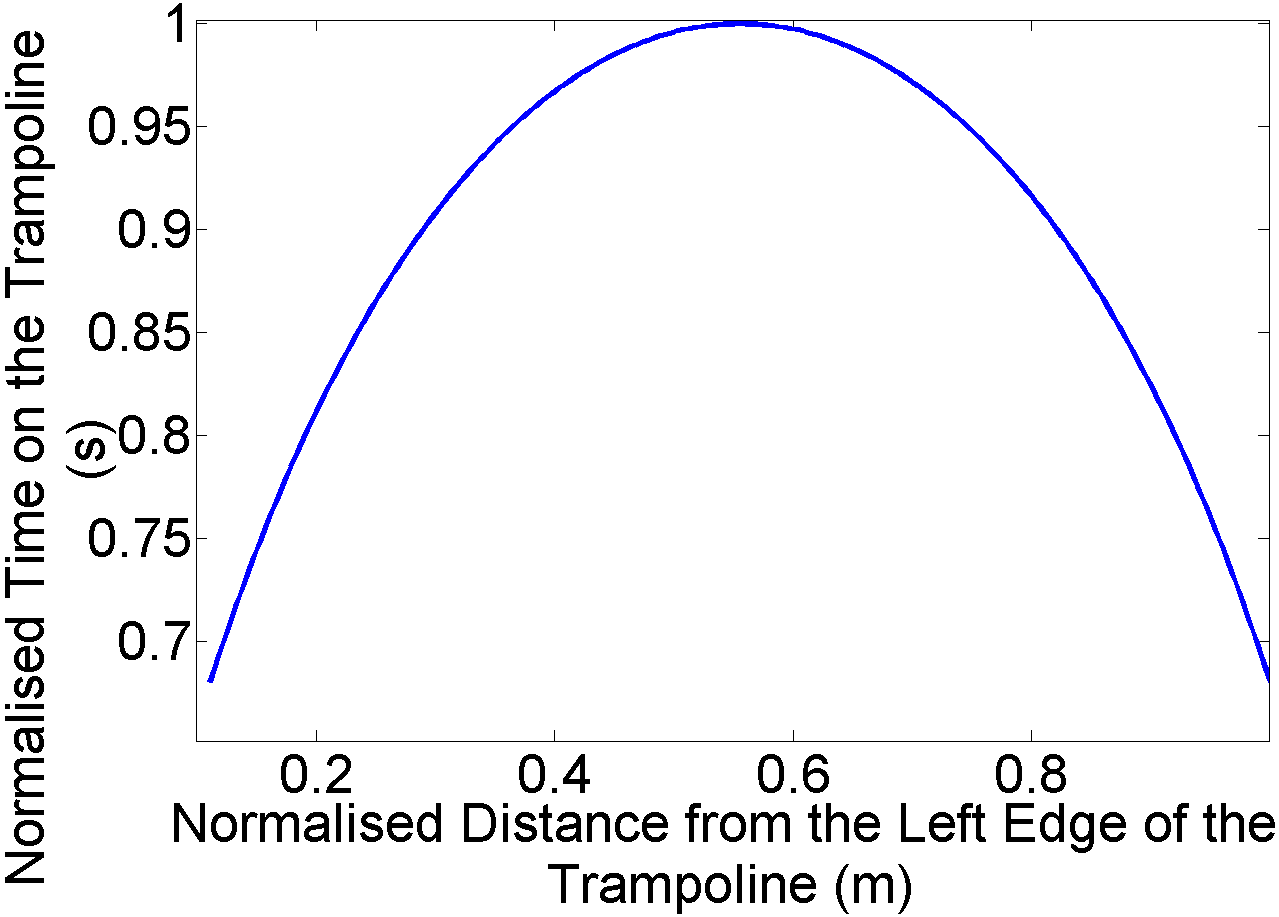
\includegraphics[width=\textwidth]{Norm_Time_DistEdge.png}
    	\caption{Time spent on trampoline.}\label{fig:Norm_Time_DistEdge}
    \end{subfigure}\hfill
	\begin{subfigure}[t]{0.3\textwidth}
		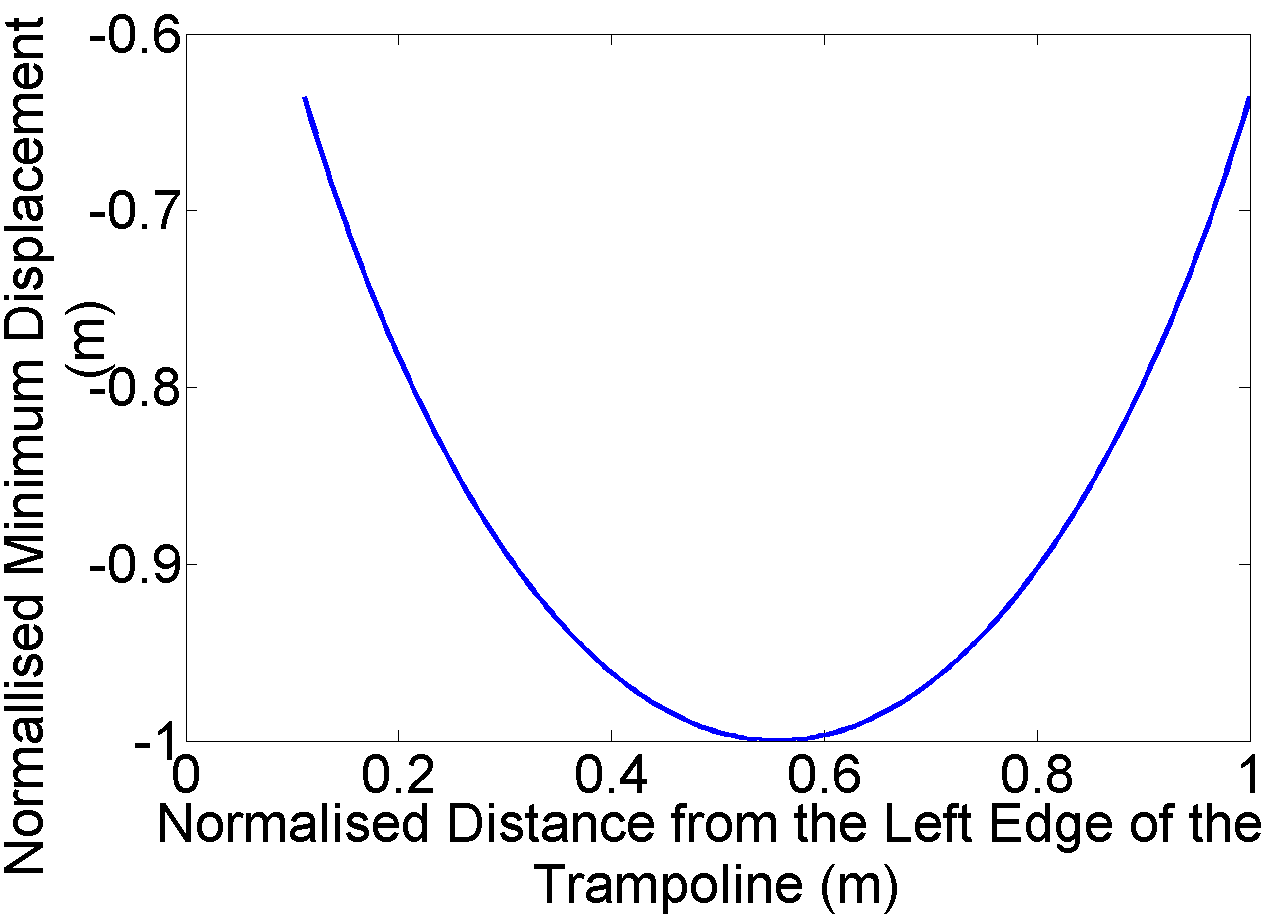
\includegraphics[width=\textwidth]{Norm_MinY_DistEdge.png}
    	\caption{Most negative displacement reached by the mass on the trampoline.}\label{fig:Norm_MinY_DistEdge}
    \end{subfigure}\hfill
    \begin{subfigure}[t]{0.3\textwidth}
		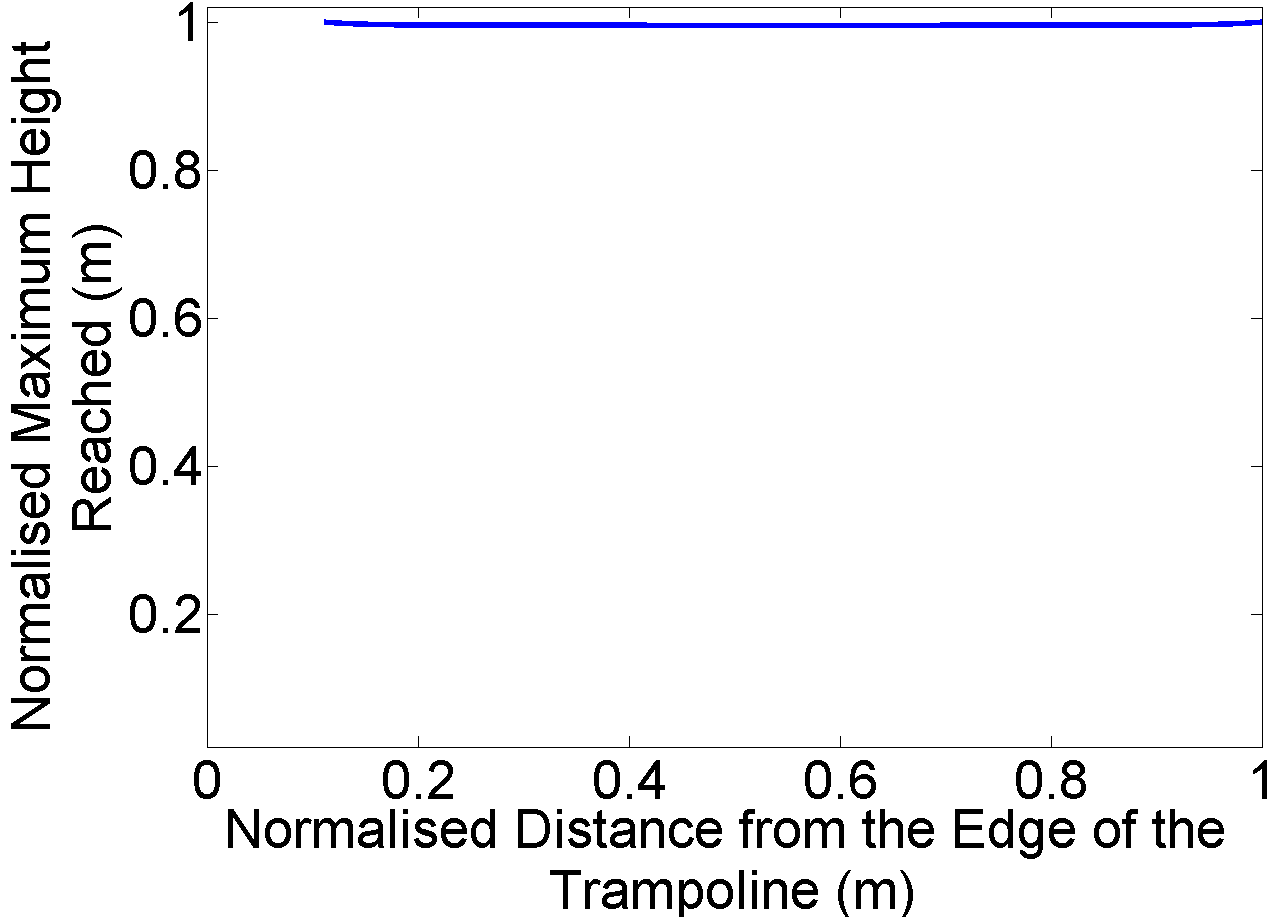
\includegraphics[width=\textwidth]{Norm_Height_DistEdge.png}
    	\caption{Maximum height reached after leaving the trampoline.}\label{fig:Norm_Height_DistEdge}
    \end{subfigure}\hfill
    \caption{The effect of the distance from the edge of the trampoline on the other parameters when kept constant.}\label{fig:Norm_DistEdge}
\end{figure}
%time
\noindent Figure \ref{fig:Norm_Time_DistEdge} shows  that the distance from the edge of the trampoline has an effect on the time spent on the trampoline.  When the mass is in the middle of the trampoline it will spends the greatest amount of time on the trampoline, and this amount of time decreases as the mass moves closer to one of the edges. This is symmetric as both spring constants are equal.
%min y
 Figure \ref{fig:Norm_MinY_DistEdge} shows that the maximum displacement occurs when the mass is placed centrally. The distribution around this point is a symmetric parabola. 
%height
The maximum height that the mass reaches when it leaves the trampoline is not effected by the distance from the edge, as can be seen in Figure \ref{fig:Norm_Height_DistEdge}. 

\paragraph{Starting Height/Velocity}\mbox{}\\

\begin{figure}[H]
	\centering
    \begin{subfigure}[t]{0.3\textwidth}
		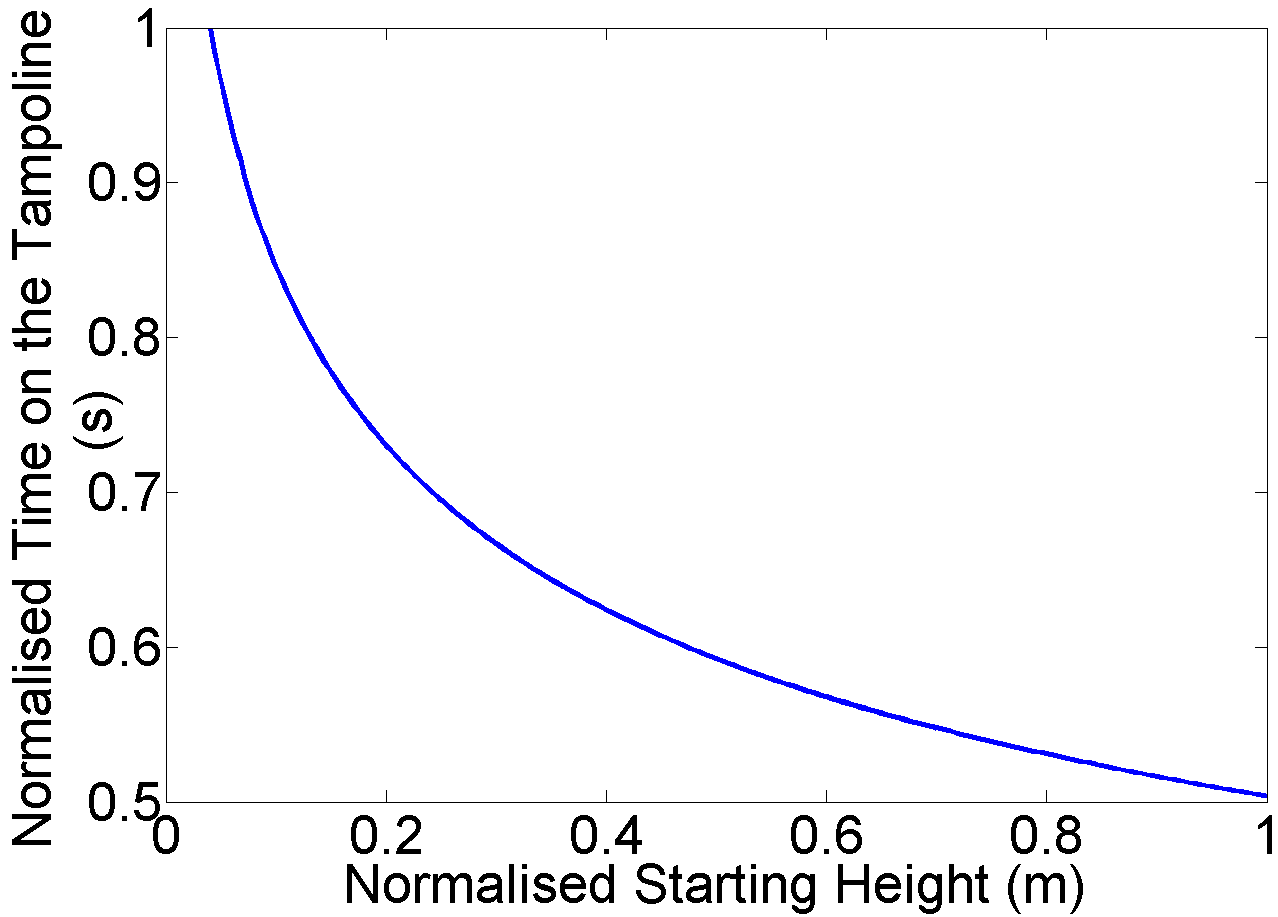
\includegraphics[width=\textwidth]{Norm_Time_StartHeight.png}
    	\caption{Time spent on trampoline.}\label{fig:Norm_Time_StartHeight}
    \end{subfigure}\hfill
	\begin{subfigure}[t]{0.3\textwidth}
		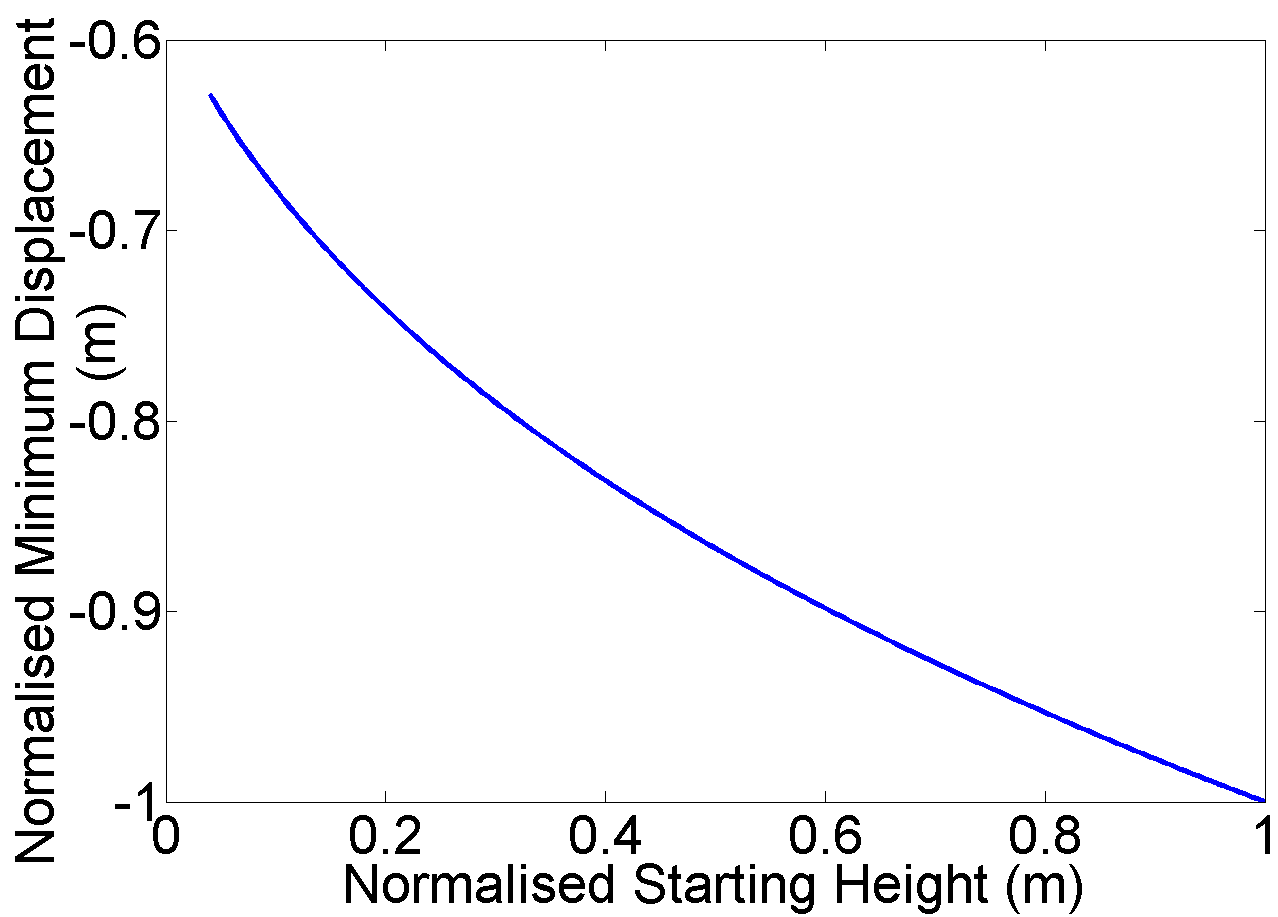
\includegraphics[width=\textwidth]{Norm_MinY_StartHeight.png}
    	\caption{Most negative displacement reached by the mass on the trampoline.}\label{fig:Norm_MinY_StartHeight}
    \end{subfigure}\hfill
    \begin{subfigure}[t]{0.3\textwidth}
		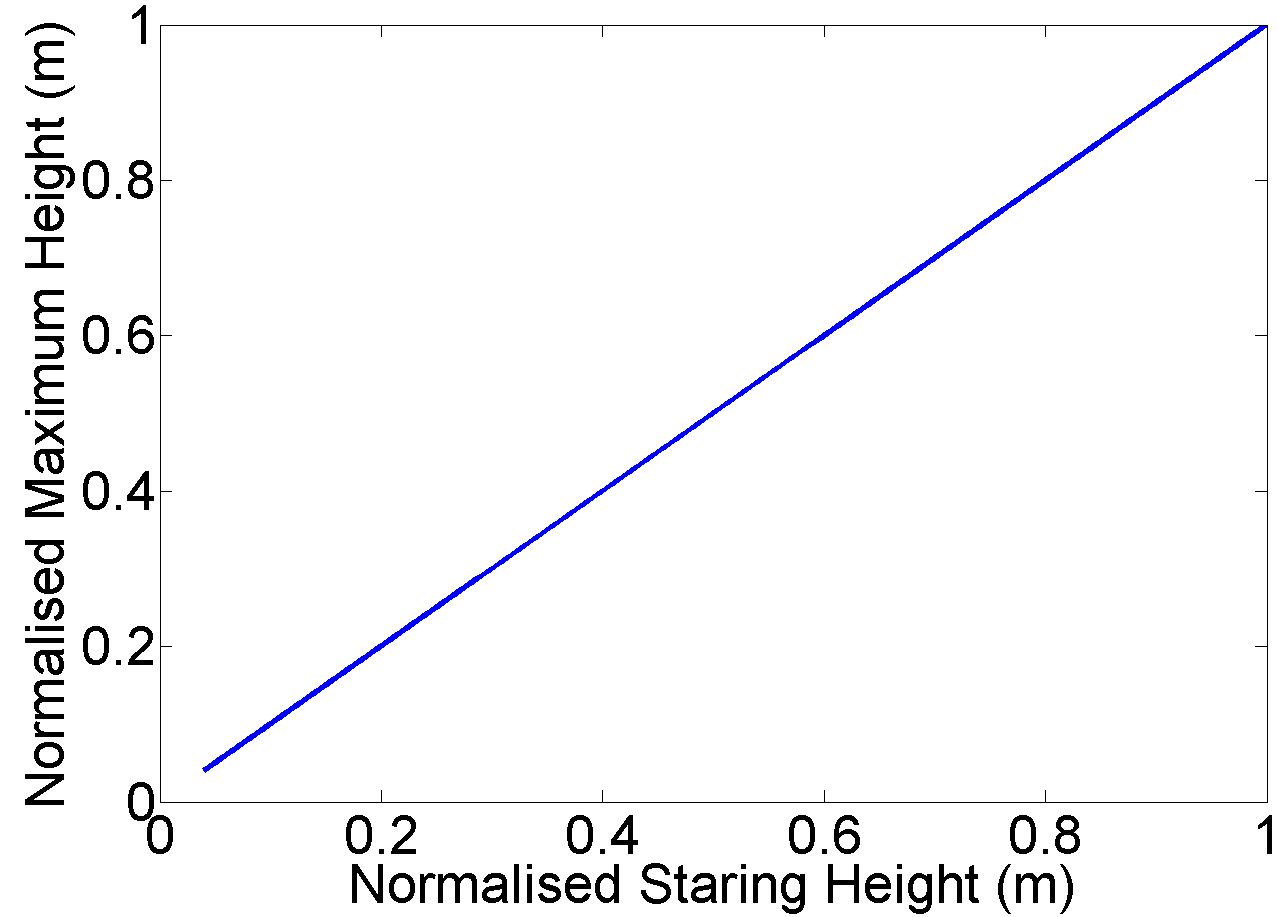
\includegraphics[width=\textwidth]{Norm_Height_StartHeight.png}
    	\caption{Maximum height reached after leaving the trampoline.}\label{fig:Norm_Height_StartHeight}
    \end{subfigure}\hfill
    \caption{How the other parameters are affected by the starting height of the mass when kept constant.}\label{fig:Norm_StartHeight}
\end{figure}
%time
\noindent As the starting height the mass is dropped from is varied the amount of time spent on the trampoline varies inverse exponentially, shown in Figure \ref{fig:Norm_Time_StartHeight}. Therefore the higher the mass is dropped from, the less time it spends attached to the trampoline.
The negative displacement reached by the mass when on the trampoline varies almost linearly as the starting height is increased, as shown in Figure \ref{fig:Norm_MinY_StartHeight}. As the starting height is increased, the finishing height also increases, seen in Figure \ref{fig:Norm_Height_StartHeight}, with a linear relationship.


\paragraph{Mass}\mbox{}\\
\begin{figure}[H]
	\centering
    \begin{subfigure}[t]{0.3\textwidth}
		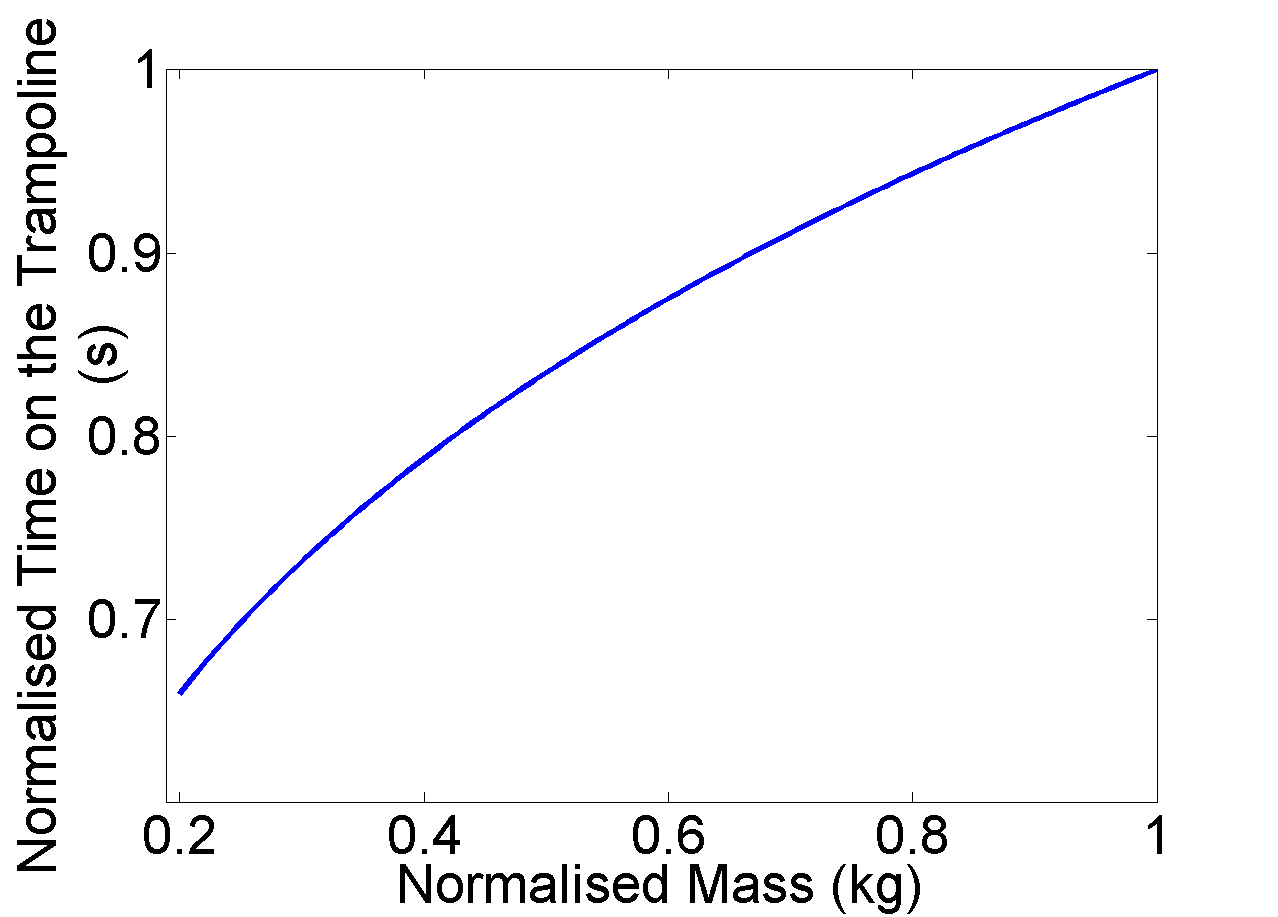
\includegraphics[width=\textwidth]{Norm_Time_Mass.png}
    	\caption{Time spent on trampoline.}\label{fig:Norm_Time_Mass}
    \end{subfigure}\hfill
	\begin{subfigure}[t]{0.3\textwidth}
		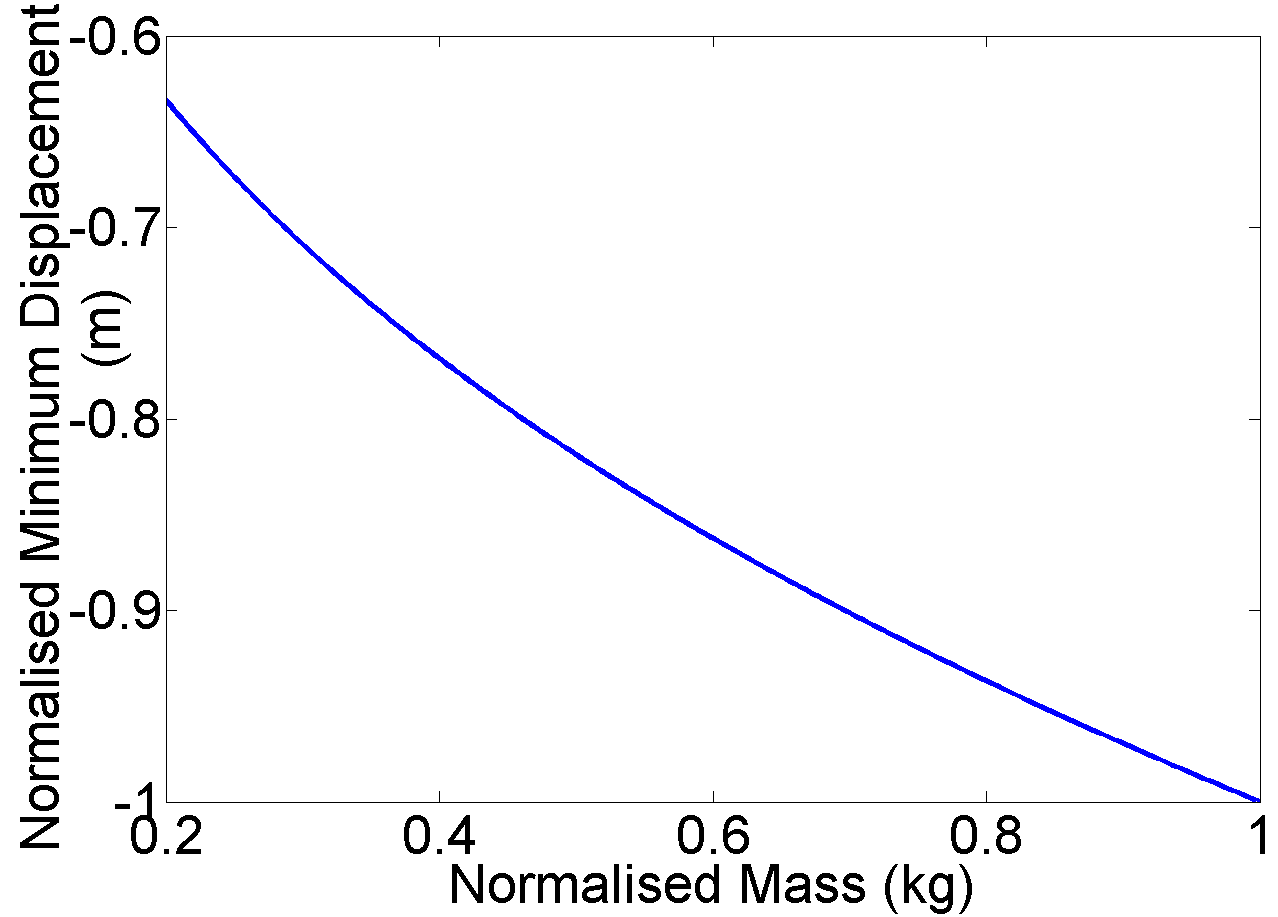
\includegraphics[width=\textwidth]{Norm_MinY_Mass.png}
    	\caption{Most negative displacement reached by the mass on the trampoline.}\label{fig:Norm_MinY_Mass}
    \end{subfigure}\hfill
    \begin{subfigure}[t]{0.3\textwidth}
		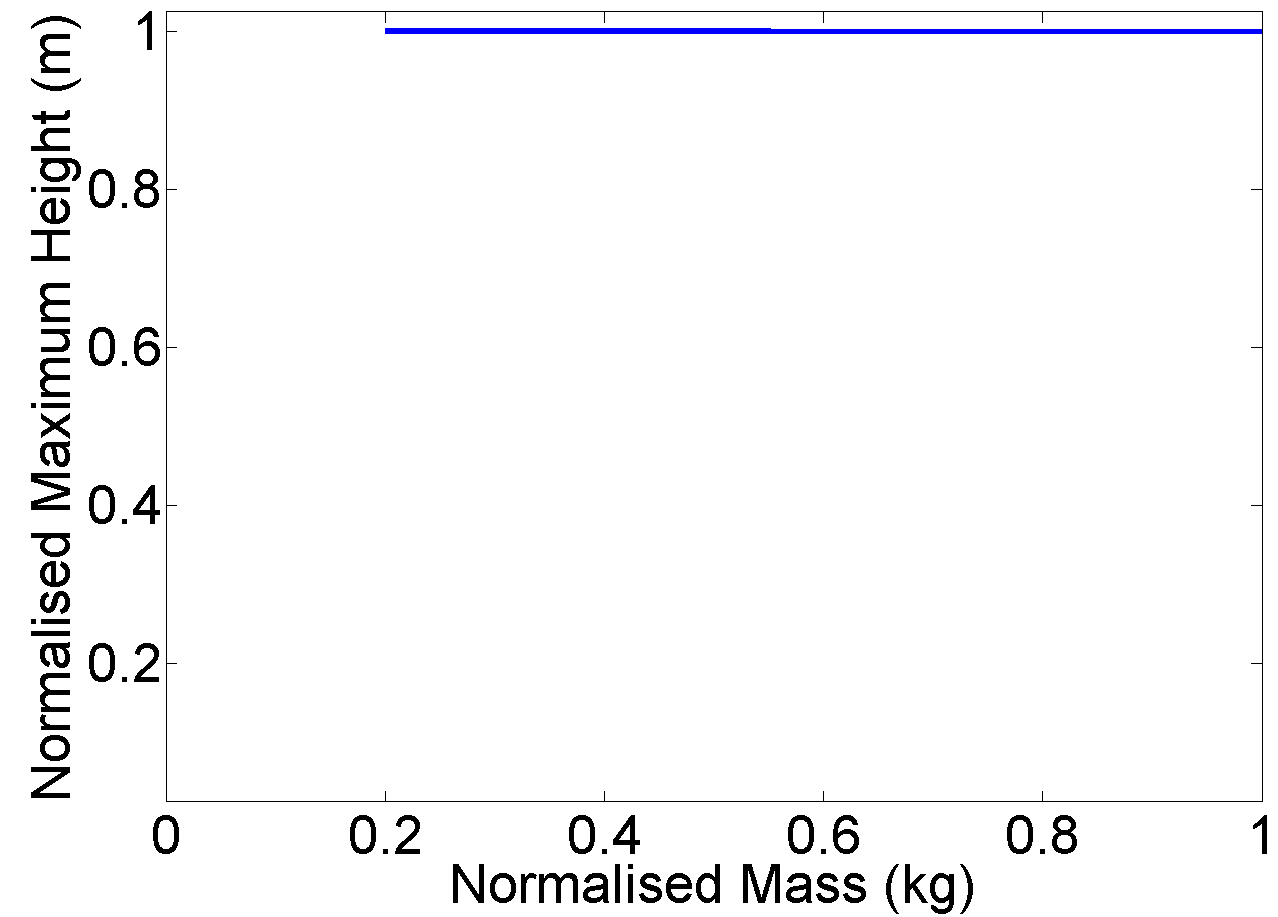
\includegraphics[width=\textwidth]{Norm_Height_Mass.png}
    	\caption{Maximum height reached after leaving the trampoline.}\label{fig:Norm_Height_Mass}
    \end{subfigure}\hfill
    \caption{How the mass of the mass affects the other parameters when kept constant.}\label{fig:Norm_Mass}
\end{figure}
%height
\noindent As the mass increases, the height that they reach from the same starting height also stays the same. This is due to the energy being conserved throughout the motion. This can be seen from Figure \ref{fig:Norm_Height_Mass}.
%min y
As the mass increases, the minimum height that it reaches decreases almost linearly, as shown by Figure \ref{fig:Norm_MinY_Mass}. This shows that the trampoline will reach a greater vertical distance the higher the mass that is used.
%time
The time spent attached to the trampoline has a positive linear relationship with the mass increasing, with Figure \ref{fig:Norm_Time_Mass} showing that the greater the mass, the more time that is spent on the trampoline.

\paragraph{Conclusions}\mbox{}\\
\noindent While the different parameters affect the total time the mass spends on the trampoline and the minimum point it reaches, the only parameter which will affect the height the mass reaches when it leaves the trampoline is the height it started at. This is to be expected because of how the conservation of energy in the Lagrangian mechanics works. So all of the kinetic energy initially put into the system will be converted into potential energy as the mass is slowed by the trampoline. It will then be converted back into kinetic energy as the mass speeds up again, leaving the trampoline with the same kinetic energy as was initially provided and therefore ending up at the height it originally started at.

\subsubsection{Video Analysis}\label{vid}
\noindent As well as being used alongside the two mass model, the one mass model was also used to find a set of parameters which produced results similar to a real life example of a person jumping on a trampoline. This provides a benchmark to compare the model to, to see how accurately it represents a real life system. In order to do this, video footage of a person falling on a trampoline was studied \cite{vidya} and a number of features were chosen for comparisons. The first feature looked at was the mass of the person, perceived to be 50kg, and the height the person fell from is also studied, which is from about 1.4m in the video. The lowest point reached when the trampoline is displaced below its starting equilibrium is found as 0.3m. The total time spent in contact with the trampoline is another feature looked at, found as 0.267s from the trampoline. Finally the maximum rebound height was found to be 0.1m from the video.\\

\noindent It is possible to find the results seen in Figure 3c by setting the following parameters to the following values:
\begin{itemize}
\item $L_1$ = 1.5m
\item $L_2$ = 1.5m
\item $k$ = 77500N/m
\item $m$ = 50kg
\end{itemize}

\noindent As can be seen, some aspects of the results are good and some are not. For example, the time spent on the trampoline was very similar to that seen in the video footage. However the minimum point reached by the mass is much lower than that seen in the video. Also, it was seen that the person jumping on the trampoline did not reach the same height they originally fell from. One reason for these discrepancies could be to do with the fact that the model created does not contain any damping, which would be present in a real life scenario. \\

\noindent Despite these discrepancies, some of these parameters were kept constant throughout the different tests carried out so that the most realistic results could be found. These were the total length of the trampoline ($L$) and the spring constants ($k$) which were 3m and 77500N/m respectively.




% \begin{figure}[H]
% 	\centering
% 	\includegraphics[width=0.6\linewidth, height=2in]{Norm-Height-StartHeight.png}
% 	\caption{Linear relationship between starting height and maximum height reached}\label{fig:normheight}
% \end{figure}

\subsection{Two Mass Model}\label{2mm}

\noindent Now that an reasonable model of a trampoline has been created, another mass can be added to the system. Interactions between the masses can be observed and information about when injury to users will occur can be gathered. \\ %edit 

\noindent The addition of a second mass to the system changes the differential equations required to simulate the system. As can be seen in Figure \ref{fig:system2} some of the parameters from the one mass model are changed and some new parameters are introduced. There is also an introduction of a second $y$ variable, so $y_1$ represents the displacement of mass $m_1$ and $y_2$ represents the displacement of mass $m_2$. \\

\begin{figure}[H]
	\centering
	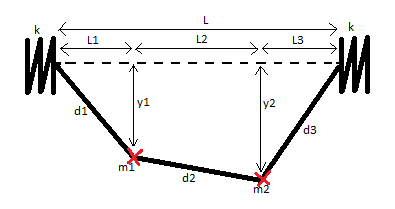
\includegraphics[width=0.6\linewidth, height=1.6in]{system2.png}
	\caption{Trampoline model with two differently weighted masses placed on it.}\label{fig:system2}
\end{figure}
% needs explaining of different lengths and why l2 is always constant.

\noindent Where:
\begin{itemize}
\item $m_1$ [kg] is the mass of one of the masses.
\item $m_2$ [kg] is the mass of the other mass.
\item $L_1$ [m] is the horizontal distance from the left spring to $m_1$.
\item $L_2$ [m] is the horizontal distance between the two masses.
\item $L_3$ [m] is the horizontal distance from the right spring to $m_2$.
\item $y_1$ [m] is the displacement of $m_1$.
\item $y_2$ [m] is the displacement of $m_2$.
\item $d_1$ [m] is the length of the string from the left spring to $m_1$.
\item $d_2$ [m] is the length of the string between the two masses.
\item $d_3$ [m] is the length of the string from the right spring to $m_2$.
\end{itemize}

\noindent For this model, parameters $L_1$, $L_2$ and $L_3$ are kept constant, allowing the remaining parameters to be found in terms of these constants and the variables $y_1$ and $y_2$. To begin with, $d_1$, $d_2$ and $d_3$ are found, as they were for the one mass model, by using Pythagoras' theorem:\\

\begin{equation}
d_1 = \sqrt{L_{1}^{2} + y_{1}^{2}} \,\,\,\,\,\,\,\,\,\,\,\,\,\,\,\,\,\,\,\,\,\,\,\,\,\,\,\,\,\,\,\,\,\,d_2 = \sqrt{L_{2}^{2} + (y_{2}-y_{1})^{2}} \,\,\,\,\,\,\,\,\,\,\,\,\,\,\,\,\,\,\,\,\,\,\,\,\,\,\,\,\,\,\,\,\,\,d_3 = \sqrt{L_{3}^{2} + y_{2}^{2}}
\end{equation}

\noindent Using the same technique as with the one mass model, the new length of the surface of the trampoline can be found by summing $d_1$, $d_2$ and $d_3$. Then, the total distance stretched by both springs is found by subtracting the distance between the springs from the new length of the surface of the trampoline. So, the distance each spring is stretched by ($\Delta x$) can be found using the following equation:

\begin{equation}
\Delta x = \frac{1}{2}\left(d_{1}+d_{2}+d_{3}-L\right)
\end{equation}

\noindent The addition of a second mass also changes the total kinetic and potential energy in the system. For this model, the two masses each provide a kinetic energy of $\frac{1}{2}m_1y_{1}^{2}$ and $\frac{1}{2}m_2y_{2}^{2}$ respectively. They also provide a gravitational potential energy of $m_1gy_1$ and $m_2gy_2$ respectively. The trampoline also provides an elastic potential of $\frac{1}{2}k\Delta x^2$. This means that:

\begin{equation}
T = \frac{1}{2}m_{1}\dot{y_{1}}^{2} + \frac{1}{2}m_{2}\dot{y_2}^{2}
\end{equation}

\noindent and

\begin{equation}
V = k\Delta x^{2} - m_{1}gy_{1} - m_{2}gy_{2} 
\end{equation}

\noindent So, using Equation (1)

\begin{equation}
L = \frac{1}{2}m_{1}\dot{y_{1}}^{2} + \frac{1}{2}m_{2}\dot{y_2}^{2} - k\Delta x^{2} + m_{1}gy_{1} + m_{2}gy_{2} 
\end{equation}

\noindent Since this system has two variables ($y_1$ and $y_2$), the Lagrange Equation (2) was used to produce two differential equations:

\begin{equation}
\frac{d}{dt}\frac{\partial \mathcal{L}}{\partial \dot{y_i}} = m_{i}\ddot{y_{i}}\,\,\,\,\,\,\,\,\,\,\,\,\,\,\,\,\,\,\,\,\,\,\,\,\,\,\,\,\,\,\,\,\,\,\,\,\,\,\,\,\,\,\,\,\,\,\,\,\,\,\,\,\,\,\,\,\, \text{for i} = 1,2
\end{equation}

\begin{equation}
\frac{\partial \mathcal{L}}{\partial y_{i}} = 2k \Delta x \frac{\partial x}{\partial y_{i}}+m_{i}g \,\,\,\,\,\,\,\,\,\,\,\,\,\,\,\,\,\,\,\,\,\,\,\,\,\,\,\,\,\,\,\,\,\, \text{for i} = 1,2
\end{equation}

\noindent Where,

\begin{equation}
\frac{\partial\Delta x}{\partial y_1} = \frac{1}{2}\left[\frac{y_{1}}{d_1} - \frac{(y_{2}-y_{1})}{d_2}\right]
\end{equation}

\begin{equation}
\frac{\partial\Delta x}{\partial y_2} = \frac{1}{2}\left[\frac{(y_{2}-y_{1})}{d_2} +\frac{y_2}{d_3} \right]
\end{equation}
\noindent Combining Equations (19),(20), (21) and (22) gives the terms for the Lagrange Equation (2):
\begin{equation}
m_{i}\ddot y_{i} + 2k\Delta x \frac{\partial \Delta x}{\partial y_{i}} - m_{i}g = 0 \,\,\,\,\,\,\,\,\,\,\,\,\,\,\,\, \text{for i} = 1,2
\end{equation}

\noindent In order to track the displacement and velocity of each of the masses from these differential equations (23), four initial conditions are required. These are the initial displacements and velocities of each of the masses. The displacement and velocity of both masses can then be tracked until one of the masses comes off the trampoline. This can be seen in Figure \ref{fig:2MM_Disp_Vel}. At this point, it is necessary to find the leaving mass. This can be found by calculating the accelerations of each mass by rearranging the differential equations (23) and using the final values found for $y_1$, $\dot{y_1}$, $y_2$, $\dot{y_2}$. The mass with an acceleration less than the acceleration due to gravity is the mass which is leaving the trampoline. Once the leaving mass has been identified, its final velocity can be used to find the maximum height reached, using equations (12) and (13). \\

\begin{figure}[H]
	\centering
    \begin{subfigure}{0.45\textwidth}
		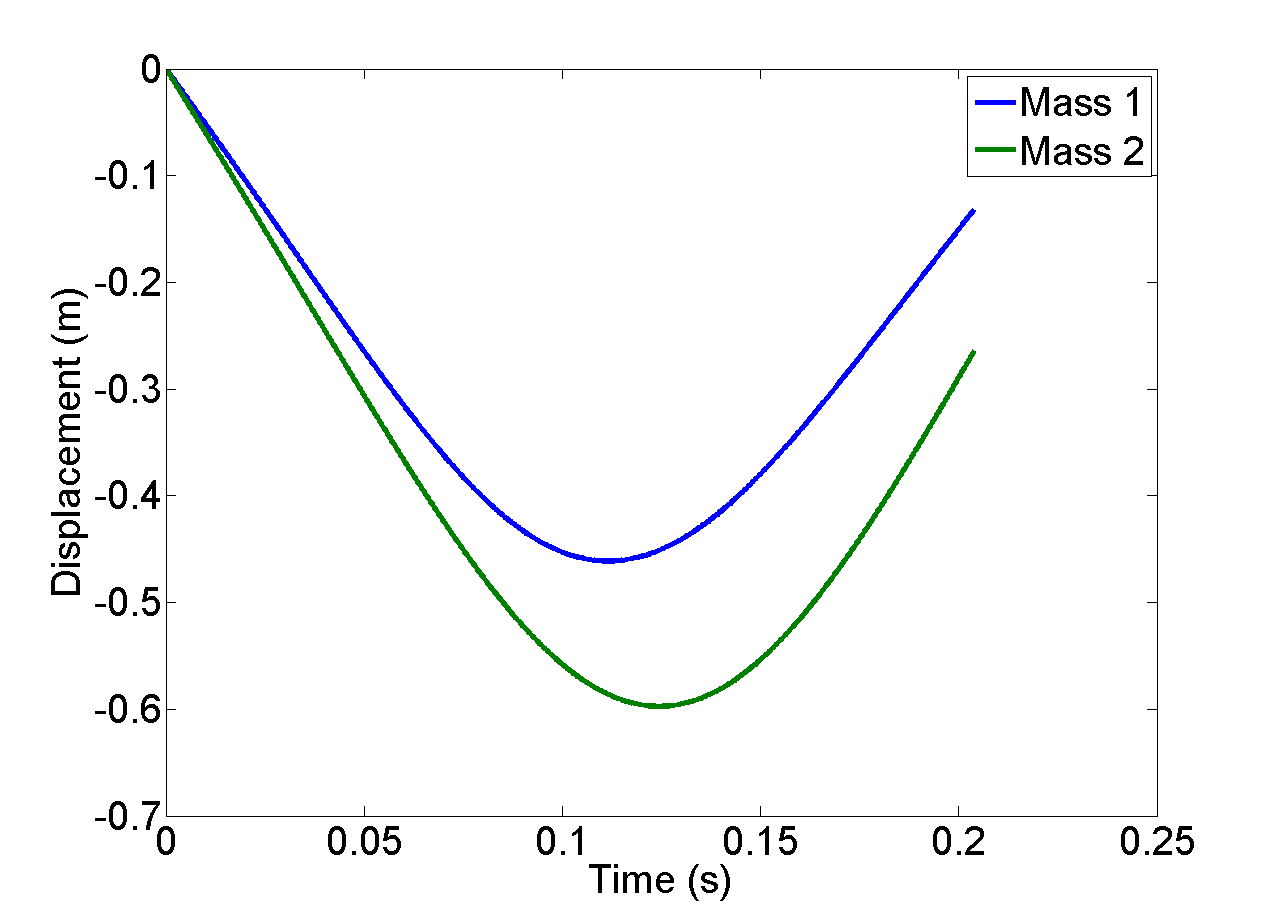
\includegraphics[width=\textwidth]{2MM_Disp.png}
    	\caption{The displacement of both of the masses while on the trampoline.}\label{fig:2MM_Disp}
    \end{subfigure}\hfill
	\begin{subfigure}{0.45\textwidth}
		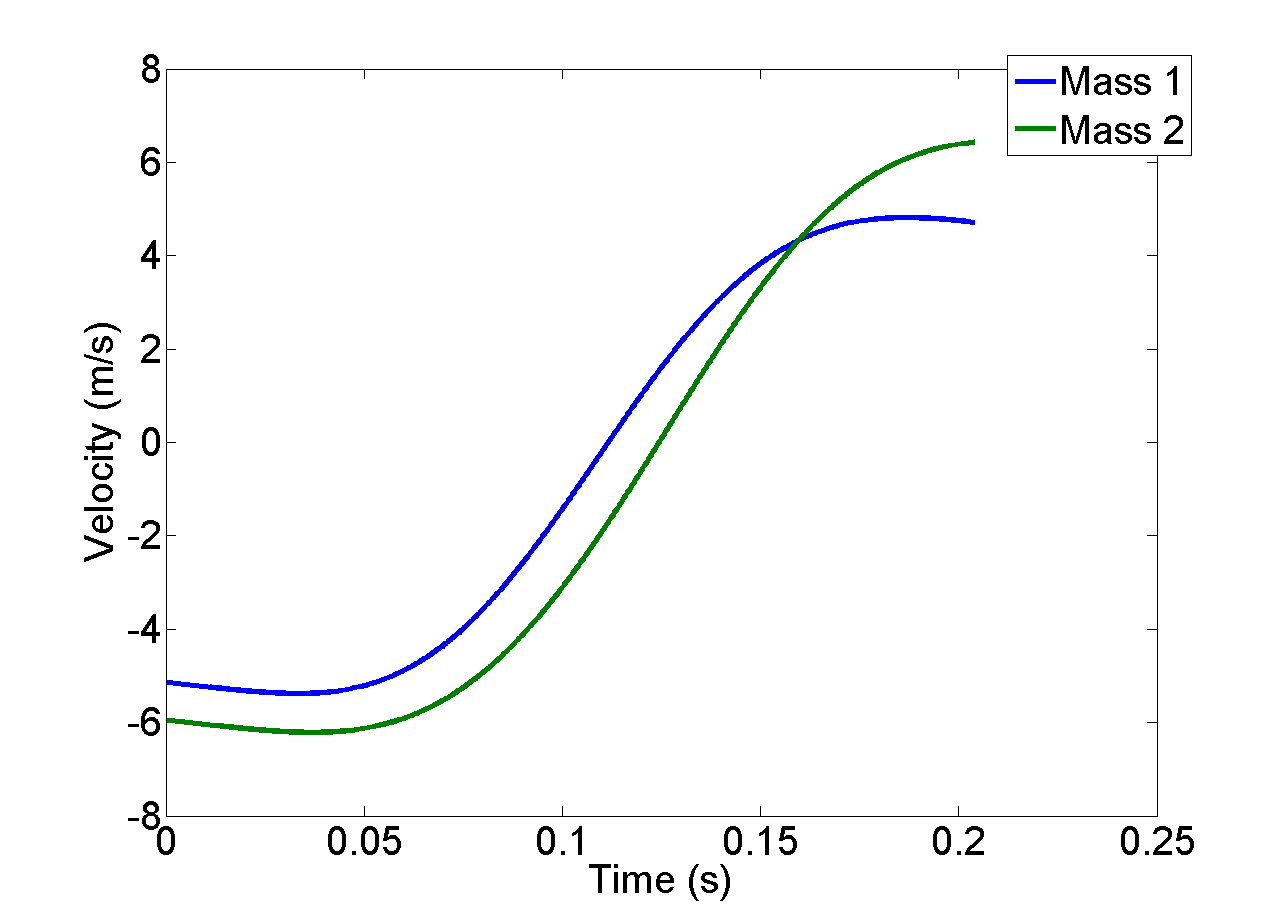
\includegraphics[width=\textwidth]{2MM_Vel.png}
    	\caption{The velocity of both of the masses while on the trampoline.}\label{fig:2MM_Vel}
    \end{subfigure}\hfill
    \caption{The displacements and velocities of a 35.6kg mass and a 70kg mass 1m apart, dropped from 1.44 and 1.8m respectively.}\label{fig:2MM_Disp_Vel}
\end{figure}

\noindent Now that two masses can be represented on a trampoline, it is possible to test the effects of changing different parameters, namely the distance between the two parameters and the time lag between the two masses coming into contact with the trampoline.

\subsection{Combining the Models}\label{combine}
%talk about how switch between 1 - 2 mass model.
In order to find the maximum heights reached by both masses for various distances between the two masses and time lags, it was necessary to combine both the one mass and two mass models. This is because the two mass model only works when both masses are on the trampoline, so the one mass model has to be used when only one of the masses is in contact.\\

\noindent Initially, the one mass model was used to find the displacement and velocity of one of the masses that is in contact with the trampoline. This will be the first mass to come into contact with the trampoline. Examples can be seen in Figure \ref{fig:dvt}. 

\begin{figure}[H]
 	\centering
	\begin{subfigure}[t]{0.45\textwidth}
		\centering
		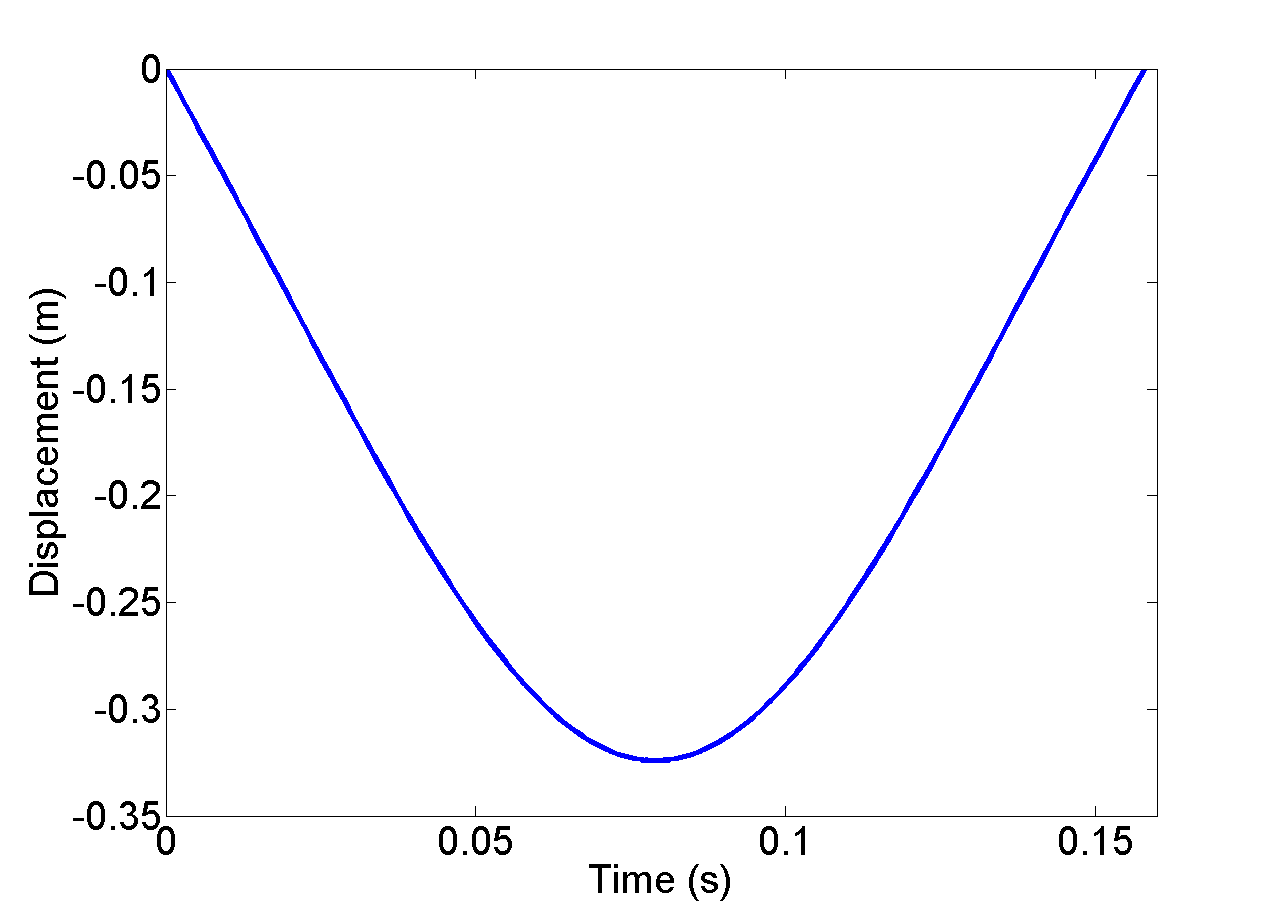
\includegraphics[width=3.1in, height=2in]{Disp_m1_144m_025fe.png}
		\caption{Displacement-Time graph for mass placed 0.25m from edge.}\label{fig:displace1}
	\end{subfigure}\hfill
	\begin{subfigure}[t]{0.45\textwidth}
    	\centering
		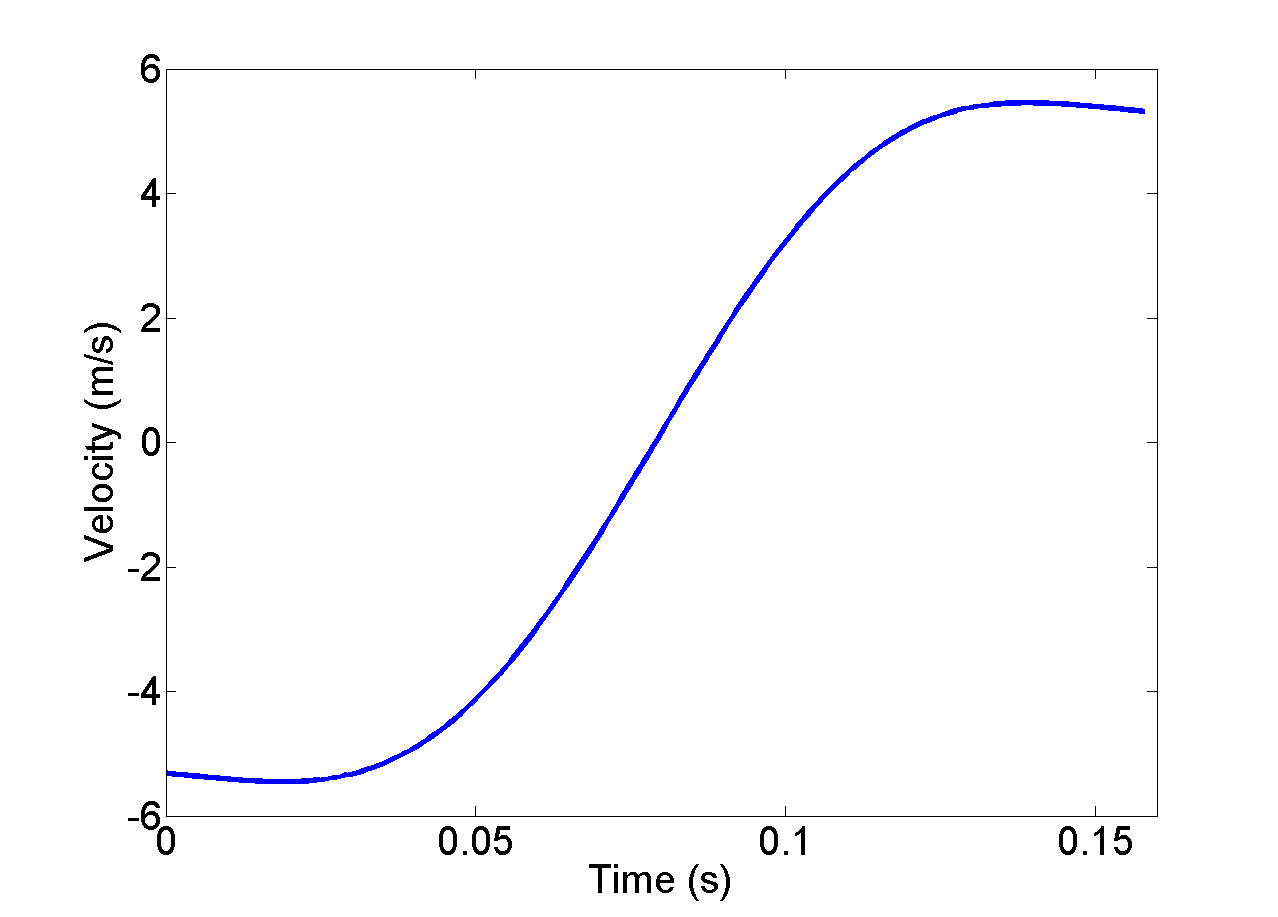
\includegraphics[width=3.1in, height=2in]{Vel_m1_144m_025fe.png}
		\caption{Velocity-Time graph for mass placed 0.25m from edge.}\label{fig:vel1}
	\end{subfigure}\hfill
     \begin{subfigure}{0.45\textwidth}
		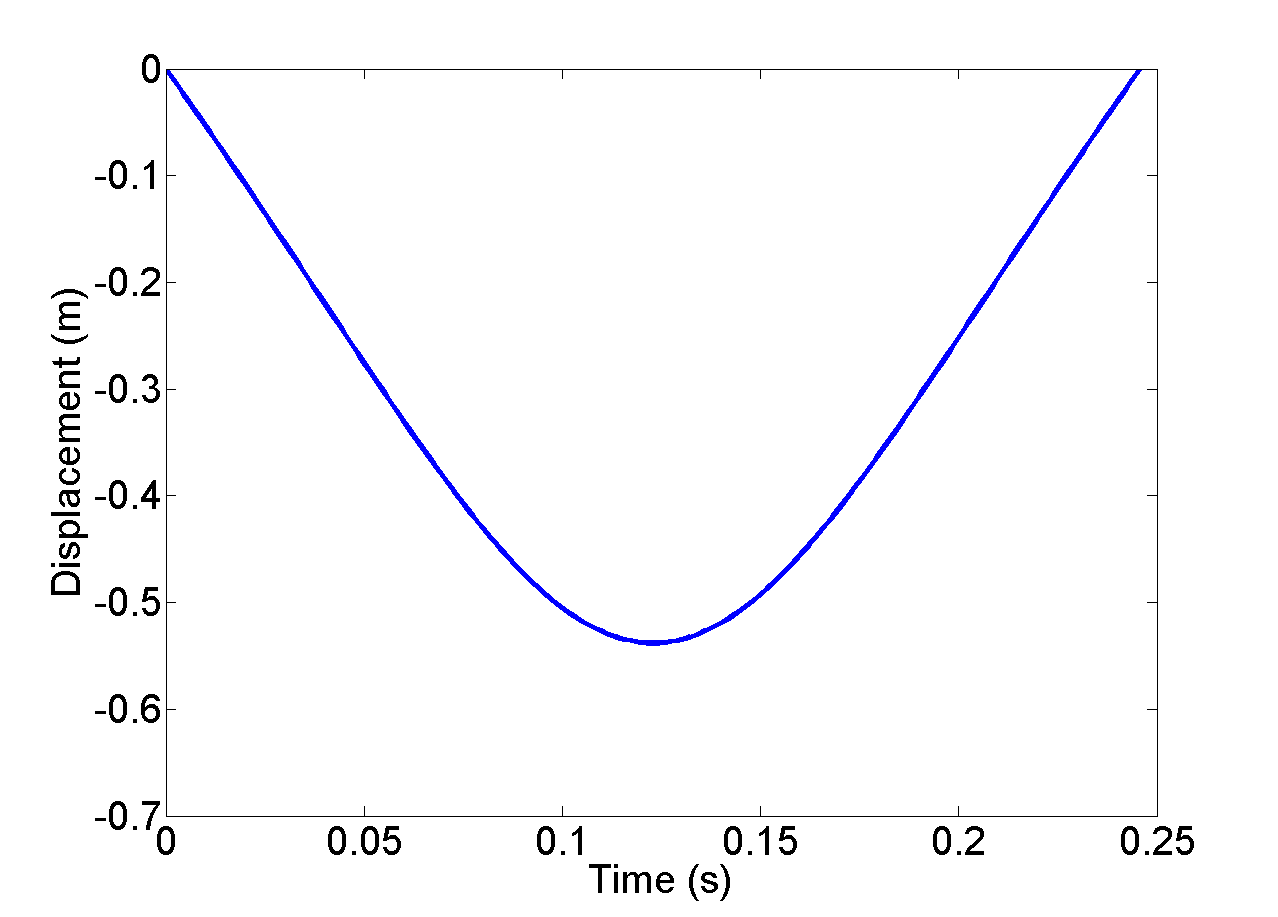
\includegraphics[width=3.1in, height=2in]{Disp_m1_144m_135fe.png}
    	\caption{Displacement-Time graph for mass placed 1.35m from edge (close to centre).}\label{fig:displace2}
    \end{subfigure}\hfill
	\begin{subfigure}{0.45\textwidth}
		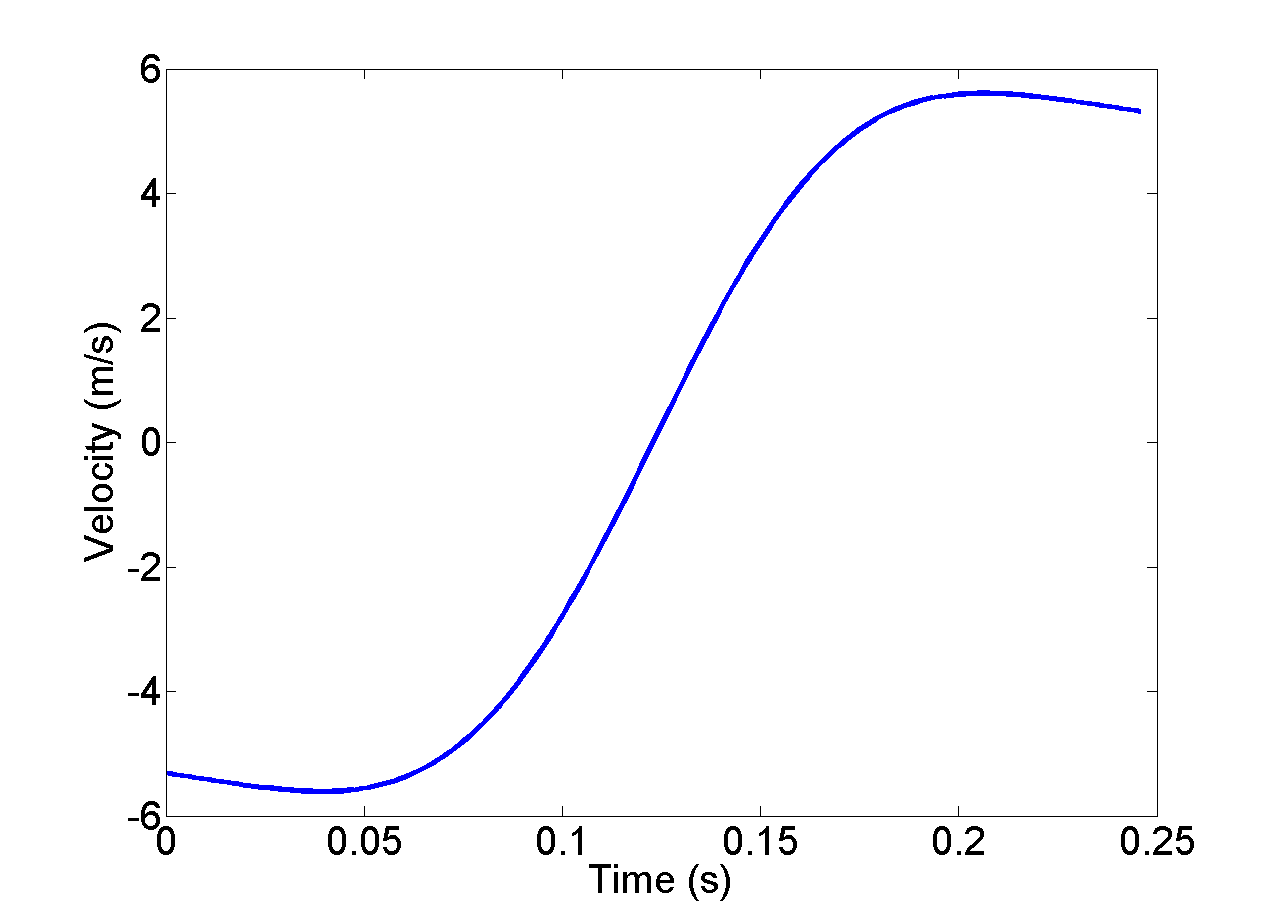
\includegraphics[width=3.1in, height=2in]{Vel_m1_144m_135fe.png}
    	\caption{Velocity-Time graph for mass placed 1.35m from edge (close to centre).}\label{fig:vel2}
    \end{subfigure}\hfill
     \caption{Graphs showing Similarities between Displacement-time and Velocity-time graphs when varying mass location on trampoline.}
   \label{fig:dvt}
\end{figure}

\noindent In order to analyse this data the way in which time is considered needs to be evaluated. Rather than looking what happens at each second, time-steps are chosen as equal fractions of the total time taken per case. For instance, both displacements, seen in Figures \ref{fig:displace1} and \ref{fig:displace2} and both velocities in Figures \ref{fig:vel1} and \ref{fig:vel2} look similar, however the time spans are different. So, by splitting the data up into time-steps, it makes it easier to draw comparisons between results while at different positions on these curves. Figure \ref{fig:displace2} plotted with 250 time-steps can be seen below in Figure \ref{fig:time_step}.% include fig


%study vt graphs for mass (central)and at (edges)
%state similarities differences
%those close to centre will fall further than those at edges
%look at total time spent on trampoline. THis differs. 
%comment on how that time scales are different but segmentation is equal( 250steps?).
% \noindent Velocity-time and displacement-time graphs from the 1 mass model when the mass is positioned close to the centre %1.35m from edge
% and when positioned close to edge %0.25m
% show little behavioural differences, shown in Figures \ref{fig:displace1}, \ref{fig:vel1}, \ref{fig:displace2} and \ref{fig:vel2} below. As expected, the mass placed centrally has a greater displacement minimum than the mass placed towards one of the edges. The most notable observation is that both results occur over different time spans. The mass placed centrally has more contact time with the trampoline, as it has further to descend and ascend.




\begin{figure}[H]
	\centering
    \begin{subfigure}{0.45\textwidth}
		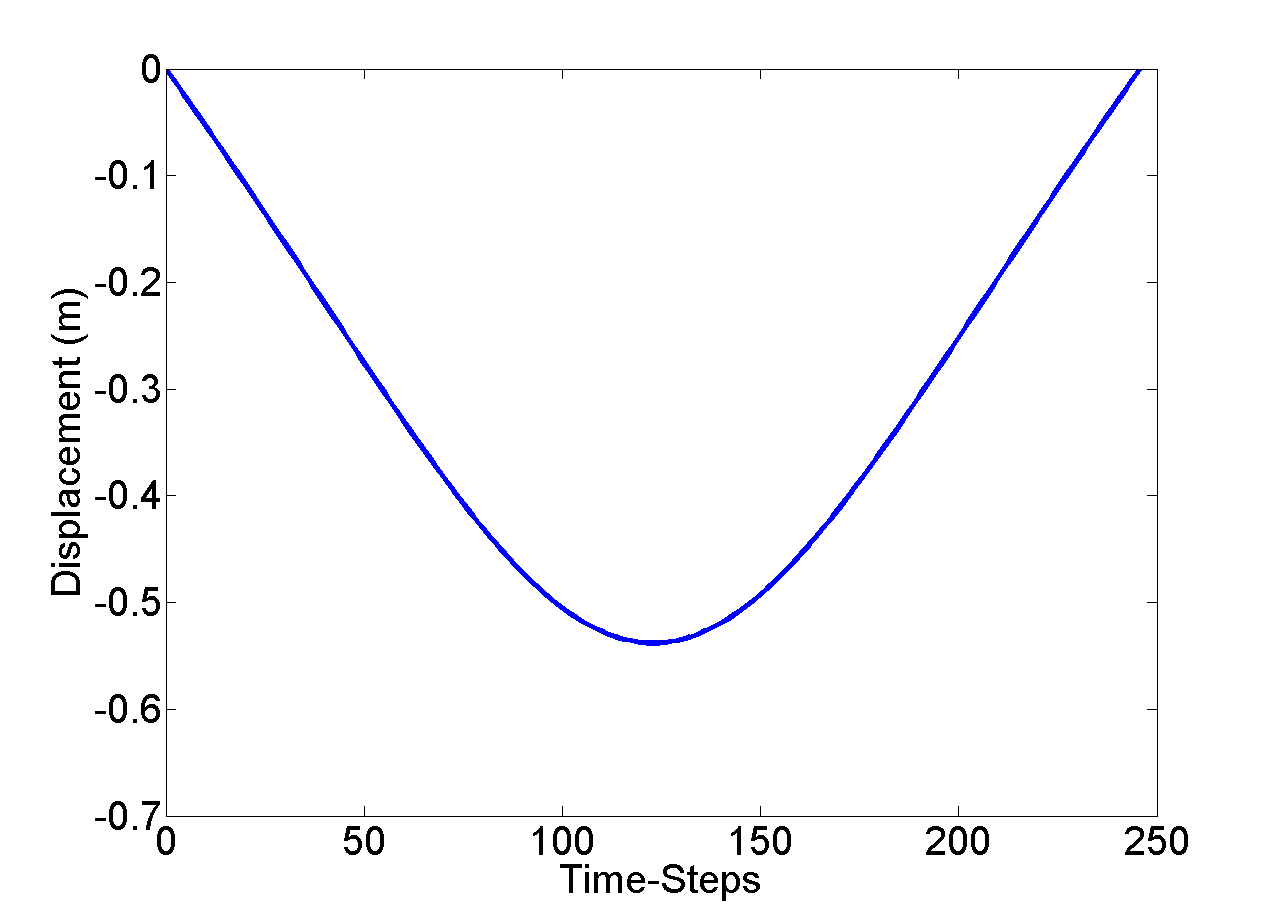
\includegraphics[width=\textwidth]{Disp_m1_144m_135fe_timesteps.png}
    	\caption{Figure \ref{fig:displace2} with time-step replacing time on the x-axis.}\label{fig:displace1_ts}
    \end{subfigure}\hfill
	\begin{subfigure}{0.45\textwidth}
		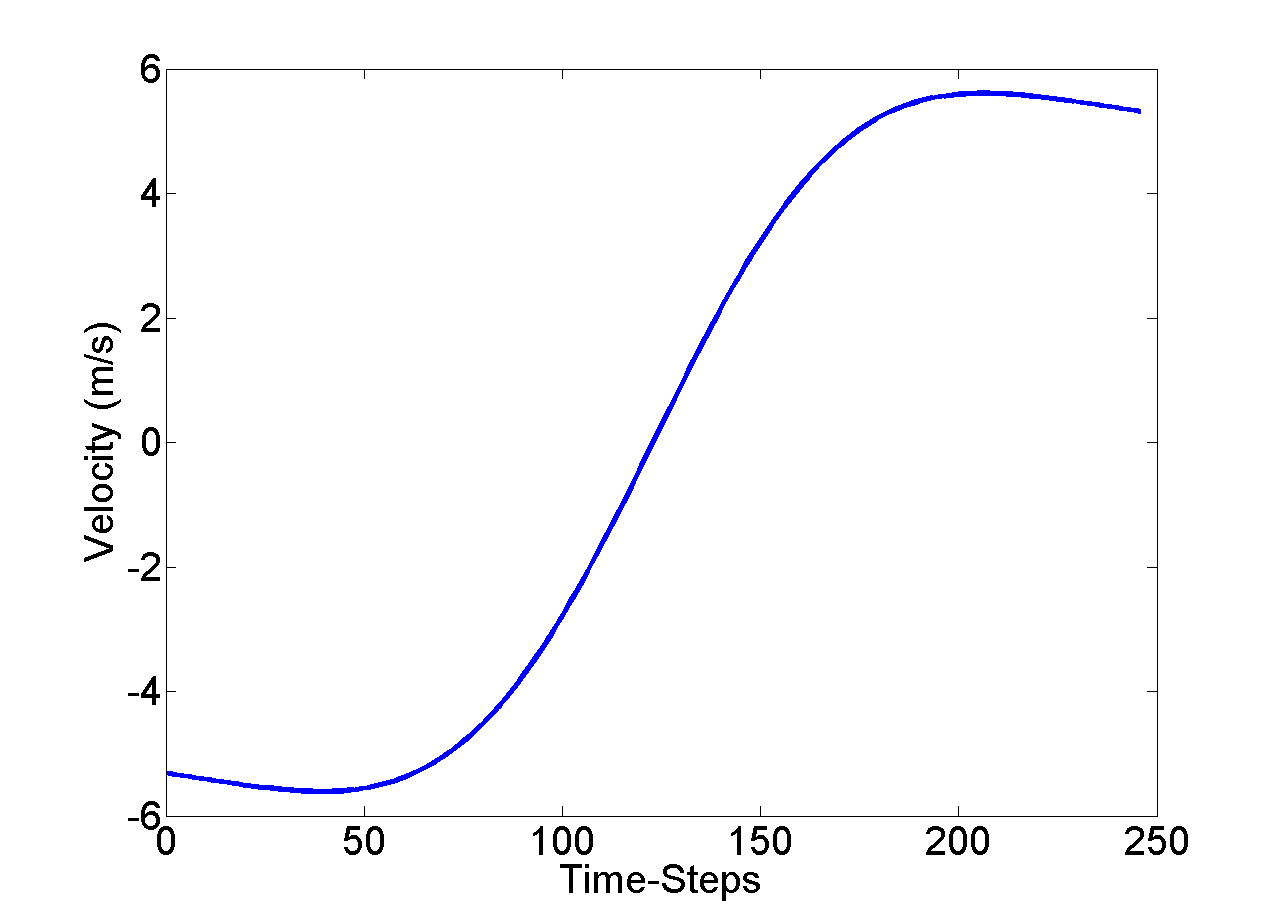
\includegraphics[width=\textwidth]{Vel_m1_144m_135fe_timesteps.png}
    	\caption{Figure \ref{fig:vel2} with time-step replacing time on the x-axis.}\label{fig:vel1_ts}
    \end{subfigure}\hfill
    \caption{Graphs showing how time-steps replace total time spent on the trampoline.}\label{fig:time_step}
\end{figure}

% \begin{figure}[H]
% 	\centering
% 	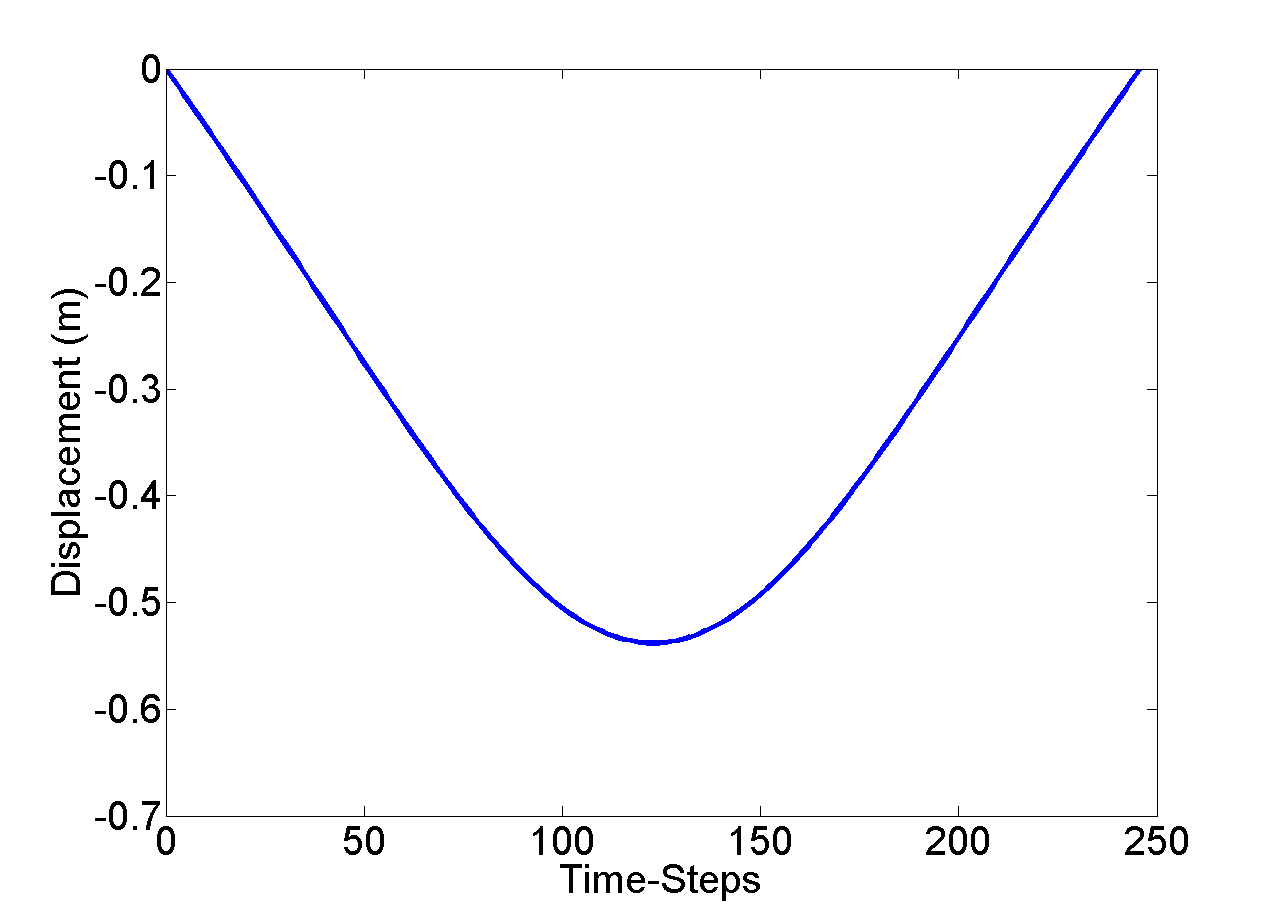
\includegraphics[width=3.1in, height=2in]{Disp_m1_144m_135fe_timesteps.png}
% 	\caption{Displacement-time-step graph for mass placed 1.35m from edge (close to centre).}\label{fig:displace2step}
% \end{figure}

\noindent For each of the time-steps of the first mass to come into contact with the trampoline, the initial conditions for the second mass being dropped onto the trampoline are calculated. These have to be calculated because the second mass is dropped from a fixed height so it will come into contact with the trampoline at different displacements and velocities depending on the displacement of the first mass on the trampoline. Once these initial condition have been found, they are combined with the conditions of the first mass on the trampoline at the relative time-step and used in the two mass model.\\

\noindent Then the results from the two mass model are taken and the maximum height of the first mass to leave the trampoline is calculated. Then the final position and velocity of the remaining mass on the trampoline from the two mass model are used as the initial conditions for the one mass model. The results from this are then found and the maximum height reached by the remaining mass is calculated. This method will only work if it assumed that the first mass to leave the trampoline does not land back on the trampoline before the second mass left.\\

\noindent This can then be repeated for various masses and distances between the masses and the results can be compared. 



%include example graph with 250 time steps.

%http://journals.plos.org/plosone/article?id=10.1371/journal.pone.0078645
%http://www.ripublication.com/ijmer_spl/ijmerv3n6spl_04.pdf
%http://aplusphysics.com/community/index.php/blog/152/entry-985-physics-of-trampolines/
%http://www.srri.umass.edu/sites/srri/files/dufresne-2001spj.pdf